\documentclass[11pt]{article}
\usepackage{graphicx}
\usepackage{amsmath}
\usepackage{fullpage}
\usepackage{amssymb}
\usepackage{amsfonts}
\usepackage{latexsym}
%\usepackage{pstricks}
\usepackage{tikz,pgflibraryplotmarks}
\usepackage{algorithm}
\usepackage{algpseudocode}
\usepackage{hyperref}
\usepackage[nottoc,numbib]{tocbibind} 
\usepackage{todonotes}
\usepackage{natbib}

\newcommand{\bfA}	{{\bf{A}}}
\newcommand{\bfB}	{{\bf{B}}}
\newcommand{\bfC}	{{\bf{C}}}
\newcommand{\bfD}	{{\bf{D}}}
\newcommand{\bfE}	{{\bf{E}}}
\newcommand{\bfF}	{{\bf{F}}}
\newcommand{\bfG}	{{\bf{G}}}
\newcommand{\bfH}	{{\bf{H}}}
\newcommand{\bfI}	{{\bf{I}}}
\newcommand{\bfJ}	{{\bf{J}}}
\newcommand{\bfK}	{{\bf{K}}}
\newcommand{\bfL}	{{\bf{L}}}
\newcommand{\bfM}	{{\bf{M}}}
\newcommand{\bfN}	{{\bf{N}}}
\newcommand{\bfO}	{{\bf{O}}}
\newcommand{\bfP}	{{\bf{P}}}
\newcommand{\bfQ}	{{\bf{Q}}}
\newcommand{\bfR}	{{\bf{R}}}
\newcommand{\bfS}	{{\bf{S}}}
\newcommand{\bfT}	{{\bf{T}}}
\newcommand{\bfU}	{{\bf{U}}}
\newcommand{\bfV}	{{\bf{V}}}
\newcommand{\bfW}	{{\bf{W}}}
\newcommand{\bfX}	{{\bf{X}}}
\newcommand{\bfY}	{{\bf{Y}}}
\newcommand{\bfZ}	{{\bf{Z}}}

\newcommand{\bfa}	{{\bf{a}}}
\newcommand{\bfb}	{{\bf{b}}}
\newcommand{\bfc}	{{\bf{c}}}
\newcommand{\bfd}	{{\bf{d}}}
\newcommand{\bfe}	{{\bf{e}}}
\newcommand{\bff}	{{\bf{f}}}
\newcommand{\bfg}	{{\bf{g}}}
\newcommand{\bfh}	{{\bf{h}}}
\newcommand{\bfi}	{{\bf{i}}}
\newcommand{\bfj}	{{\bf{j}}}
\newcommand{\bfk}	{{\bf{k}}}
\newcommand{\bfl}	{{\bf{l}}}
\newcommand{\bfm}	{{\bf{m}}}
\newcommand{\bfn}	{{\bf{n}}}
\newcommand{\bfo}	{{\bf{o}}}
\newcommand{\bfp}	{{\bf{p}}}
\newcommand{\bfq}	{{\bf{q}}}
\newcommand{\bfr}	{{\bf{r}}}
\newcommand{\bfs}	{{\bf{s}}}
\newcommand{\bft}	{{\bf{t}}}
\newcommand{\bfu}	{{\bf{u}}}
\newcommand{\bfv}	{{\bf{v}}}
\newcommand{\bfw}	{{\bf{w}}}
\newcommand{\bfx}	{{\bf{x}}}
\newcommand{\bfy}	{{\bf{y}}}
\newcommand{\bfz}	{{\bf{z}}}

\newcommand{\A}		{\vec{A}}
\newcommand{\B}		{\vec{B}}
\newcommand{\C}		{\vec{C}}
\newcommand{\D}		{\vec{D}}
\newcommand{\E}		{\vec{E}}
\newcommand{\F}		{\vec{F}}
\newcommand{\G}		{\vec{G}}
\renewcommand{\H}	{\vec{H}}
\newcommand{\I}		{\vec{I}}
\newcommand{\J}		{\vec{J}}
\newcommand{\K}		{\vec{K}}
\renewcommand{\L}	{\vec{L}}
\newcommand{\M}		{\vec{M}}
\newcommand{\N}		{\vec{N}}
\renewcommand{\O}	{\vec{O}}
\renewcommand{\P}	{\vec{P}}
\newcommand{\Q}		{\vec{Q}}
\newcommand{\R}		{\vec{R}}
\renewcommand{\S}	{\vec{S}}
\newcommand{\T}		{\vec{T}}
\newcommand{\U}		{\vec{U}}
\newcommand{\V}		{\vec{V}}
\newcommand{\W}		{\vec{W}}
\newcommand{\X}		{\vec{X}}
\newcommand{\Y}		{\vec{Y}}
\newcommand{\Z}		{\vec{Z}}

\newcommand{\hf}        {{\frac 12}}
\newcommand{\bfepsilon} {{\boldsymbol \epsilon}}
\newcommand{\bfsigma}   {{\boldsymbol \sigma}}
\newcommand{\bfSigma}   {{\boldsymbol \Sigma}}
\newcommand{\bfOmega}   {{\boldsymbol \Omega}}
\newcommand{\bfomega}   {{\boldsymbol \Omega}}
\newcommand{\bfGamma}   {{\boldsymbol \Gamma}}
\newcommand{\bfgamma}   {{\boldsymbol \gamma}}
\newcommand{\bfPhi}     {{\boldsymbol \Phi}}
\newcommand{\bflambda}  {{\boldsymbol \lambda}}
\newcommand{\bfmu}      {{\boldsymbol \mu}}
\newcommand{\bfeta}     {{\boldsymbol \eta}}
\newcommand{\bftau}      {{\boldsymbol \tau}}
\newcommand{\bfupsilon}      {{\boldsymbol \upsilon}}
\newcommand{\bnabla}	 { { \boldsymbol \nabla} }
\newcommand{\btheta}	 { { \boldsymbol \theta} }
\newcommand{\balpha}	 { { \boldsymbol \alpha} }
\newcommand{\bfxi}		 { { \boldsymbol \xi} }
\newcommand{\bfdelta}	 { { \boldsymbol \delta} }



\newcommand{\LtL}       { \bfL^{\top}\bfL}

\newcommand {\vu}  	 {{\vec {\bf  u}} }   
\newcommand {\vuref} {\vu_{\text{ref}}}  
\newcommand {\vq}  	 { {\vec {\bf  q}} }
\newcommand {\ve}    { {\vec {\bf  e}} }
\newcommand {\vh}    { {\vec {\bf  h}} }
\newcommand {\vx}    {\vec {\bf x}}     
\newcommand {\bx}    {{\bf{x}}}   
\newcommand {\zero}  { {\bf 0} }

\renewcommand{\hf}		 {\frac12}
\newcommand{\hx}[1]		 {{\ensuremath{h^x_{\scriptscriptstyle #1}}}}
\newcommand{\hy}[1]		 {{\ensuremath{h^y_{\scriptscriptstyle #1}}}}
\newcommand{\hz}[1]		 {{\ensuremath{h^z_{\scriptscriptstyle #1}}}}


\newcommand{\s}		{\vec{s}}
\newcommand{\h}		{\vec{h}}
\newcommand{\n}		{\vec{n}}
\newcommand{\x}		{\vec{x}}
\renewcommand{\u}		{\vec{u}}
\renewcommand{\div}	{\nabla\cdot\,}
\newcommand{\grad}	{\ensuremath {{\bf{ \nabla}}}}
\newcommand{\curl}	{\ensuremath{{\nabla}\times\,}}
\newdimen\iwidth\iwidth=30mm
\newcommand{\rottext}[1]	{\rotatebox{90}{\hbox to 30mm{\hss #1\hss}}}
\newcommand{\rme}			{\rm{e}}
\newcommand{\HRule}			{\rule{\linewidth}{0.25mm}}

\newcommand{\JJ} 	 {\mathcal{J}}    % objective functional
\newcommand{\cD} 	 {\mathcal{D}}    % data misfit
\newcommand{\CR} 	 {\mathcal{R}}    % regularization functional
\newcommand{\CRflow} {\mathcal{R}^{\text{flow}}}    %  flow 
\newcommand{\CRsat}  {\mathcal{R}^{\text{s}}}     %  saturation 
\newcommand{\CF} 	 {\mathcal{F}}    % continuous tomography operator
\newcommand{\sh} 	 {\texttt{s}}     % discretized initial slowness
\newcommand{\DIVh}   {{\textsf{DIV}}}  % discretized divergence 
\newcommand{\CURLh}  {{\textsf{CURL}}} % discrete curl operator
\newcommand{\GRADh}  {{\textsf{GRAD}}} % discrete gradient operator

\newcommand{\bfmhat}    {{\widehat{\bfm}}}
\newcommand{\bfdhat}    {{\widehat{\bfd}}}
\newcommand{\bfwhat}	{\widehat{\bf w}}

\newcommand*\xbar[1]{%
  \hbox{%
    \vbox{%
      \hrule height 0.5pt % The actual bar
      \kern0.5ex%         % Distance between bar and symbol
      \hbox{%
        \kern-0.em%      % Shortening on the left side
        \ensuremath{#1}%
        \kern-0.15em%      % Shortening on the right side
      }%
    }%
  }%
} 
\newcommand{\mbar}	{\xbar{\bf m}}
\newcommand{\wbar}	{\xbar{\bf w}}
\newcommand{\dbar}	{\xbar{\bf d}}
\newcommand{\Fbar}	{\xbar{\bf F}}
\newcommand{\diag}	{\sf diag}
\def\kronecker{\raisebox{1pt}{\ensuremath{\:\otimes\:}}} 











\sloppy



\begin{document}

\title{ Adaptive A-optimal experimental design for dynamical systems}
\author{J. Fohring and E. Haber }
\maketitle


\begin{abstract}
The optimal collection of data required to infer dynamic model parameters governing a time dependent partial differential equation (PDE) through the inversion process is important to may applications, particularly as it can reduce subsequent costs by reducing total measurements. 
 Popular methods which reduce the number of data required seek a set of measurements which minimize the mean square error (mse)  of the estimated model parameters. For linear ill-posed model estimation problems, these methods depend only on the physics of the problem and information provided through regularization. Thus historic data are not included, nor does the design necessarily track the dynamic target.

 To include prior data in the design process, we reformulate the model estimation inverse problem to include both the dynamic PDE and historic data. We present two model estimation formulations based on the classification of the error in the dynamic process, and then define  adaptive optimal design, which minimizes the adapted  mean square error (amse) of the estimated models. The amse is defined such that historic model estimates are included in the model optimization problem through a monitor function. This monitor function depends on prior model estimators and scales the mse such that areas of interest  contribute  to the design. In this way, minimizing the amse in the design optimization problem results in designs where historic  data and the dynamics contribute to the design of the future experiment.

We demonstrate the adaptive optimal design method for a two dimensional target whose motion is governed by a tracer advection model, and where a seismic borehole tomography survey was used to image the target in the subsurface. Using this model we show that the adaptive design method produces designs which track the motion of the target with a  significantly reduced set of data. 
 


\end{abstract}


\section{Introduction}

 While there exists a vast area of research and development in optimal experimental design for well posed inverse problems with static targets, there is little in the way of optimal design algorithms for ill-posed inverse problems where the forward problem is governed by a dynamic system. Although static design methods can be applied to time dependent PDE's as in \cite{Alexanderian2014},this approach results in experimental designs for ``all times'' which are dependent only on prior information provided in the form of a regularization (or prior) to the ill-posed problem.
 In many realistic scenarios, after a first experiment is conducted, the available data contain valuable information about the target to be recovered. This information should thus be included in the design algorithm for the future experiments. In this paper we present an adaptive method to determine an optimal experimental design for a dynamic system given historic data.
 
There are several considerations to be made when developing an optimal experimental design method. One such item is what exactly is meant by an 'optimal experiment'. In our context we refer to the problem of determining  the optimal placement of sensors to infer model parameters  through the inversion of  data. 
 Although there are several design criteria for such inverse problems, standard references for well-posed optimal experimental designs include \cite{Fedorov1972,Atkinson1992,Banks2011,Verdinelli2013}, we focus on A-optimal design in our work. 
 \begin{itemize}
 
\item Optimal design for geophysical imaging (tomography, em, and gw hydrology) \cite{Curtis1999,Ajo-Franklin2009,Coles2009a,Hus1989,Maurer2000,Wilkinson2012} 

\item Optimal design for ill-posed problems \cite{Bardow2008,Haber2008,Lucero2013}
 \end{itemize}
 The A-optimal design method minimizes the mean squared error (mse) of the posterior model estimator, or the trace of the posterior covariance matrix (from the Bayesian perspective), associated with the posterior probability law for the parameter field solution to a governing linear partial differential equation. Here our work builds on A-optimal design algorithms presented in \cite{Haber2011} for large-scale ill-posed inverse problems, and on work presented in \cite{Fohring2014} where both a static imaging PDE and the dynamic PDE describing the motion of a target were combined such that the dynamic model parameters could be inferred from imaging data. 

One major challenge when combing PDE's to formulate an inverse problem is how to characterize the error. One approach, as in \cite{Fohring2014} is to group or ignore the error in the dynamic PDE and formulate the problem as a PDE constrained optimization problem. This approach was also demonstrated in  \cite{Alexanderian2014}, where designs were computed for all times for a advection-diffusion model.  A second approach is to consider a formulation where the error in the dynamics are accounted for in a similar fashion to a linear Kalman filtering formulation \cite{Kalman1960}. We will address both cases in this work. However, in either case the mse of the inferred model parameters does not depend on historic data, only on a-priori information. To incorporate historic data into the A-optimal design algorithm we will instead compute a post-priori design, where we define the adapted mean square error  (amse) by introducing a monitor function dependent on historic estimates of the  target. 

The idea of a-priori verses post-priori  estimators is not new. For example, in adaptive mesh refinement, when numerically 
solving partial differential
equations one often uses a-priori estimates in order to solve the problem on one mesh 
and then refines the mesh in order to obtain a more accurate solution \cite{Multigrid}. The posterior estimate thus contributes to the decision as to where to refine the mesh. In our case we will apply a similar logic to influence the design algorithm in such a way that we design for the dynamic target model parameters. 

\bigskip

The paper is outlined as follows. In section \ref{sec: Adaptive} we derive from first principals the mse of a linear estimator, then present the adapted mse and define its monitor functions. In section \ref{sec:Dynamic} we briefly outline the two methods for combining two different PDEs governing the imaging technique and the dynamic motion, and present the adaptive design algorithms.  
In section \ref{sec:Opt} we outline the numerical optimization method for solving the design problem, and finally in sections \ref{sec: Example1} and \ref{sec:Results} we present  numerical examples demonstrating the adaptive A-optimal design method. 




\section{ Adaptive experimental design }
\label{sec: Adaptive}
To present the adaptive experimental design method we begin by deriving A-optimal design from first principals.

 Consider the case where we have a time dependent measurement of the form
\begin{eqnarray}
\label{data}
\bfF_{1} \bfm + \bfepsilon_1 = \bfd_{1}\quad {\rm and} \quad \bfF_{2} \bfm + \bfepsilon_2 = \bfd_{2}
\end{eqnarray}
where $\bfF_{1}$ is the forward operator at time $t_{1}$ and $\bfF_{2}$ is the forward operator 
at time $t_{2}$.
Our goal is to design the experiments at times $t_{1}$ and $t_{2}$ such that we obtain the ``best''
recovery by some criteria.

Two different designs can be considered. First, it is possible to perform {\em a-priori} design, that is,
to design the experiments $\bfF_{1}$ and $\bfF_{2}$ prior to the data collection. This is the case
when the time between $t_{1}$ and $t_{2}$ is much shorter than the time for the processing
of the data. A second approach is to use {\em post-priori} design. The idea here is to use the 
results obtained from the first experiment in order to design a ``better'' second experiment.
Our goal is to first obtain an a-priori design for the first experiment
and then, after the data is collected and processed, use the estimator
obtained at $t_{1}$ in order  to design the data collection
at time $t_{2}$.

Before we discuss the design of the data acquisition for time $t_{2}$
 we review the a-priori design of the experiment at time $t_{1}$. Our approach is based
 on the  A-optimal design criteria, which is now derived from first principles.
 
Consider  the estimation of $\bfm$ given $\bfd_{1}$, which is accomplished by solving the ill-posed optimization problem
\begin{eqnarray*}
\label{mest1}
\hf \| \bfF_{1} \bfm - \bfd_{1}\|^{2}_{\bfW_{1}} + {\frac {\alpha} 2}
\|\bfL (\bfm - \bfmhat_{0}) \|^{2}_2. 
\end{eqnarray*}
where $\bfW_{1} = {\sf diag}(\bfw_{1})$ is a matrix of inverse standard deviations, 
that is, the inverse covariance of the noise.
Minimizing the  optimization problem yields the estimator
\begin{eqnarray}
\label{mest}
\widehat \bfm_{1} = (\bfF_{1}^{\top} \bfW_{1}\bfF_{1} + \alpha \bfL^{\top} \bfL)^{-1} (\bfF_{1}^{\top} \bfW_{1} \bfd_{1}
+ \alpha \LtL \bfmhat_{0}).
\end{eqnarray}
Defining the matrix $\bfC = (\bfF_{1}^{\top} \bfW_{1}\bfF_{1} + \alpha \LtL)$, and recalling that $\bfF_1\bfm + \bfepsilon_1 = \bfd_1$ we can write
the error in the recovery as
\begin{eqnarray}
\bfmhat_1 -\bfm &=& \bfC^{-1} \bfF_{1}^{\top} \bfW_{1}\bfF_{1} \bfm + \bfC^{-1} \bfF_{1}^{\top} \bfW_{1}\bfepsilon_1 + \alpha
\bfC^{-1} \LtL \bfmhat_{0} \\
\nonumber
&+& (\alpha \bfC^{-1} \LtL\bfm
- \alpha \bfC^{-1} \LtL \bfm) 
 -\bfm.
\end{eqnarray}
Collecting terms and using the definition of $\bfC$ we obtain
\begin{eqnarray}
\label{diffmod}
\bfmhat_1 -\bfm = \bfC^{-1} \bfF_{1}^{\top} \bfW_{1} \bfepsilon_1 + \alpha \bfC^{-1} \LtL (\bfmhat_{0} - \bfm).
\end{eqnarray}
Squaring and taking the expectation over $\bfepsilon_1$ and recalling that $ \bfepsilon_1 \sim N(\zero,{\sf cov}(\bfepsilon_1) = \bfW_{1}^{-1}$, we obtain that the mean square error is
\begin{eqnarray}
{\sf mse}(\bfw,\bfm) = \bfE\| \bfmhat_1 -\bfm \|^{2} = {\sf trace}[   \bfF_{1} \bfC^{-2} \bfF_{1}^{\top} \bfW_{1}]  + 
\alpha^2 \bfE\| \bfC^{-1} \LtL (\bfmhat_{0} - \bfm) \|^{2}.
\end{eqnarray}
If we assume that $\bfm-\bfm_{0}$ is Gaussian with a zero mean and a covariance
$(\alpha \LtL)^{-1}$ then we obtain that
\begin{eqnarray}
\phi(\bfw_1 ) = {\sf mse}(\bfw_1) = {\sf trace}[    \bfC^{-2} \bfF_{1}^{\top}\bfW_{1}\bfF_{1}]  + 
 \alpha {\sf trace} [\bfC^{-2} \LtL] . 
\end{eqnarray}
Finally, using the linearity of the trace and the definition of $\bfC$ we obtain that
\begin{eqnarray}
\label{design1}
\phi_{1}(\bfw_1 ) =  {\sf trace} \left[   (\bfF_{1}^{\top}\bfW_{1}\bfF_{1}   + 
 {\alpha} \LtL)^{-1} \right]. 
\end{eqnarray}
In the design problem we seek to obtain a better estimate for $\bfm$ and therefore
we minimize $\phi_{1}(\bfw_{1})$ with an additional cost on $\bfw_{1}$, for example, in our
previous work we proposed to minimize the function
\begin{eqnarray}
\label{designp1}
\phi_{1}^{\beta}(\bfw_1 ) =  {\sf trace} \left[   (\bfF_{1}^{\top}\bfW_{1}\bfF_{1}   + 
 {\alpha} \LtL)^{-1} \right]  + \beta \sum \bfw_{1} \quad \quad 0 \le \bfw 
\end{eqnarray}
which balances the minimization of the least square error and the cost of the experiment \cite{Haber2008}.


\bigskip

Consider now using the design problem of estimating $\bfm$ given the estimated model $\widehat \bfm_{1}$.
One could rewrite the recovery problem in a similar way, that is
\begin{eqnarray}
\label{mest2}
\hf \| \bfF_{1} \bfm - \bfd_{1}\|^{2}_{\bfW_{1}} + \hf \| \bfF_{2} \bfm - \bfd_{2}\|^{2}_{\bfW_{2}}  + {\frac {\alpha} 2}
\|\bfL (\bfm -\bfmhat_{0}) \|^{2}_2. 
\end{eqnarray}
which leads to the estimate

\begin{eqnarray}
\label{mest2}
\bfmhat_{2}(\bfw_{2}) = (\bfF_{1}^{\top} \bfW_{1}\bfF_{1} +
\bfF_{2}^{\top} \bfW_{2}\bfF_{2} + \alpha \LtL)^{-1} (\bfF_{1}^{\top} \bfW_{1} \bfd_{1} +\bfF_{2}^{\top} \bfW_{2} \bfd_{2}
+ \alpha \LtL \bfmhat_{0})
\end{eqnarray}
Note that we assume that $\bfw_{1}$ is fixed and therefore the new estimate is a function of $\bfw_{2}$ alone.
If we repeat the steps above then we obtain that the A-optimal design for time $t_{2}$ yields the minimization of
the function
\begin{eqnarray}
\label{design2na}
\phi_{2}(\bfw_{2} ) =  {\sf trace} \left[   (\bfF_{1}^{\top}\bfW_{1}\bfF_{1}   + \bfF_{2}^{\top}\bfW_{2}\bfF_{2} +
\alpha \LtL)^{-1} \right]. 
\end{eqnarray}
While this design optimization problem can be solved, it does not take into consideration the fact that 
we already  have an estimate of the model, $\bfmhat_{1}$ and therefore, does not include the 
information we have already obtained at time $t_{1}$ in order to plan a better design.
It is easy to verify that any linear estimator of the data yields a covariance matrix that is independent of $\bfd_{1}$,
and therefore the approach above does not yield a post-priori estimator.


In order to use the information obtained at time $t_{1}$ for the design of the experiment at time $t_{2}$
 we now present the concept of {\em adaptive design}.

 Assume that the model, $\bfmhat_{1}$ has some ``interesting'' features and some ``boring'' features.
For example, assume that the difference
\begin{eqnarray*}
\label{diff}
 \bfdelta_{1} = \bfmhat_{1} - \bfmhat_{0}
\end{eqnarray*}


is small in some norm over some region and large in others. The goal then is to better estimate the new features
that appear in the model. It may also be the case that we wish to design only for the new best estimate of $\bfm$, $\bfmhat_1$ itself. This implies that $\bfm_0=0$. 

To this end, we introduce a {\bf monitor function}, $\bftau(\bfdelta)$ that measures
the change in the model. 
Examples for this function are
\begin{subequations}
\label{taufuns}
\begin{eqnarray*}
\bftau_{s} &=& \bfdelta \odot \bfdelta \\
\bftau_{B} &=& 
\begin{cases}
0, & \text{if } \bfdelta \leq 0\\
1, & \text{if } \bfdelta > 0
\end{cases}
\end{eqnarray*}
\end{subequations}
but other functions can be used. The first monitor  function, $\tau_{s}$, simply measures the change in the estimator
compared to the a-priori information in a 2-norm, while the second, $\tau_{N}$, is a binary function which evenly measures those changes. 

Given the monitor function,
rather than minimizing the mean square error, we propose to minimize the
adaptive mean square error, ${\sf amse}$ defined by
\begin{eqnarray}
\label{amse}
{\sf amse}(\bfw,\bfm) = \| \bfmhat_2 -\bfm \|_{\bftau_1}^{2} = 
 (\bfmhat_2 -\bfm)^{\top}{\sf diag}(\bftau_1)(\bfmhat_2 -\bfm).
 \end{eqnarray}
The idea behind the {\sf amse} is to obtain a tighter bound on the model where the estimator exhibits large changes
compared to the known a-priori estimator. 

Starting from  equation \eqref{diffmod}, modifying it to deal with the {\sf amse}, and repeating the calculation above we obtain that the expectation 
over the {\sf amse} is
\begin{eqnarray}
\label{design2ad}
\phi_{2}(\bfw_{2}) =  {\sf trace} \left[  {\sf diag}(\bftau) (\bfF_{1}^{\top}\bfW_{1}\bfF_{1}   + \bfF_{2}^{\top}\bfW_{2}\bfF_{2} +
\alpha \LtL)^{-1} \right]. 
\end{eqnarray}
Similar to the non-adaptive case, the adaptive design is obtained by minimizing the (penalized) 
function $\phi_{2}(\bfw_{2})$.

In general, the design for the k$^{th}$ experiment given data collected for times $t_1,..t_{k-1}$ is
\begin{eqnarray}
&&\phi_{k}(\bfw_{k}) =  {\sf trace} \left[  {\sf diag}(\bftau_{k-1}) \Big(\sum_{j=1}^{k}\bfF_{j}^{\top}\bfW_{j}\bfF_{j}   +
\alpha \LtL\Big)^{-1} \right]\\
&&\bftau_{k-1}(\bfmhat_{k-1}-\bfmhat_{k-2})\\
&& \bfmhat_{k-1} ={\sf argmin } \;\; \hf  \sum_{j=1}^{k-1}\| \bfF_j\bfm - \bfd_j \|^2_2 + R(\bfm).
\end{eqnarray}
If the model $\bfm$ is a dynamic target, then some consideration must be made as to how the dynamics are incorporated. 

\section{Dynamic target}
\label{sec:Dynamic}
In the previous section we presented a formulation for adaptive A-optimal experimental design that incorporates historic data given a set of measurements. However, we did not distinguish between a static model $\bfm$  or a model that is changing over time.
To design for a moving target, we must address how the dynamics describing its motion are defined. 

Consider the discrete  dynamic process and imaging  described  by the following set of linear equations
\begin{subequations}
\begin{eqnarray}
\label{eq:dynamic}
\bfm _k&=& \bfT\bfm_{k-1} + {\bfeta}_k,\\
\label{eq:image}
\bfd_k &=& \bfF \bfm_k + {\bfepsilon}_k,
\end{eqnarray}  
\end{subequations}
where the transport matrix $\bfT: \mathbb{R}^{N} \rightarrow \mathbb{R}^{N}$  is a discretization of the PDE governing the dynamics in the system. The noise vectors $\bfeta_k $ and $\bfepsilon_k $ are assumed to be Gaussian normal, $\bfeta_k \sim N(\bfeta_0,\bfQ_k)$ and ${\bfepsilon_k} \sim N(\bfepsilon_0,\bfW^{-1}_k)$.

In combining equations \eqref{eq:dynamic} and \eqref{eq:image}  there are two instances of the dynamics that result in different formulations. These are  whether there is noise in the equations describing the motion or not, $\bfeta_k \overset{?}{=} \zero$. We present differing formulations  for  the so called noiseless case $\bfeta = \zero$, and the noisy case $\bfeta \neq \zero$ in the following sections.

\subsection{Noiseless model dynamics}
Setting $\bfeta_k = \zero$ allows us to write the model at time $t_k$ as a linear mapping of the initial model $\bfm_0$, such that
\begin{eqnarray*}
\bfm_{k} &=& \bfT\bfm_{k-1}, \;\;\;{\sf or } \\
\bfm_{k} &=& \bfT^{k-1}\bfm_0.
\end{eqnarray*} 
To this end the data for time step $t_k$ can be written in terms of the initial model 
\begin{equation}
\bfd_k = \bfF_k\bfm_0 + \bfepsilon_k
\end{equation}
where $\bfF_k = \bfF\bfT^{k-1}$, and the estimation of the initial model $\bfm_0$ given $k$ data sets is 
\begin{equation}
\bfmhat_{0,k} ={\sf argmin } \;\; \hf  \sum_{j=1}^{k}\| \bfF\bfT^{j-1}\bfm_0 - \bfd_j \|_{\bfW_j}^2 + \frac{\alpha}{2}\|\bfL\bfm_0\|_2^2.
\end{equation}
Substituting the definition of $\bfF_k$ into the {\sf amse} leads to the {\sf amse} design functional,
\begin{equation}
\label{eq:noiselessPhi}
\phi_{k}(\bfw_{k}) = {\sf tr} \left[  {\sf diag}(\bftau) \Big(\sum_{j=1}^{k}(\bfF\bfT^{j-1})^{\top}\bfW_{j}\bfF\bfT^{j-1}   +
\alpha \LtL \Big)^{-1} \right] .
\end{equation}

In minimizing equation \eqref{eq:noiselessPhi} a sparsity penalty, $\beta\|\bfw_k\|_1$, is imposed on the weight vector to guarantee a design with a minimal number of measurements. Additionally we require that the weights all be positive, as it does not make sense to have negative variances. The adaptive design optimization problem is then
\begin{eqnarray}
\label{eq:noiselessOpt}
\nonumber
 &&\min_{\bfw_k}\;\;\Bigg \{\text{tr}\Big[ {\sf diag}(\bftau) \Big(\sum_{j=1}^{k}\bfF_{j}^{\top}\bfW_{j}\bfF_{j}   +
\alpha \LtL\Big)^{-1}\Big] + \beta \bfe^{\top}\bfw_k \Bigg \}\\
 &&\text{ s.t.} \;\;\;0 \geq \omega_i,
\end{eqnarray}
where $\bfe$ is a vector of ones (the constraint allows us to write the 1-norm as a sum). 

\bigskip
The adaptive design method is outlined in  algorithm \ref{algo1} below.
\begin{algorithm}
\caption{Adaptive Optimal Design: Noiseless dynamics}\label{algo1}
\begin{algorithmic}[1]
%1
\State Given a prior $\bfmhat_{0}$  for $\bfm$, set $\bftau(\bfmhat_0)$
\Comment{if there is no prior, $\bftau = \bfI$}
%2
\For{$k = 1 \text{ to } n$}  
\Comment{ $n$ time points}
%3
\State $\bfw_{k} = {\sf argmin }\;\;\ \phi_k(\bfw_k) + \beta\bfe^{\top}\bfw_k$ \Comment{design using equation \eqref{eq:noiselessPhi}} 
%4
\State Given $\bfw_k$ collect data $\bfd_k$
%
%5
\State $\bfmhat_{0,k} ={\sf argmin } \;\; \hf  \sum_{j=1}^{k}\| \bfF\bfT^{j-1}\bfm_0 - \bfd_j \|^2_2 + R(\bfm_0)$
\Comment {re-estimate $\bfm_0$ }
%6
\State $\bftau(\bfmhat_{0,k})$
\Comment Recompute the monitor function $\bftau$
\EndFor
%%%%%%%%%%%%%%%%%%%%%%%%%%%%%%%%%%%%%%%%%%%%%%%%%%%%%%%%%%%%%%%%%%%%%%%%%%%%%%%%%%%%%%
\end{algorithmic}
\end{algorithm}
Note that in step 5 of the algorithm we have left the regularization as an arbitrary function even though the design functional was derived for a linear regularization. The regularization adjusts the ill-posed inverse problem such that the solutions best estimate the true model parameter distributions, so when calculating the monitor function it is imperative to get a best estimate since this directly effects the experimental design. For example, one could choose total variation as a regularization to promote sharper edges then say the smoothing gradient operator if this is expected of the model. 
\subsection{Noisy model dynamics}
\label{sec:Noisy}
To include the noise inherent in the dynamic model we begin by  considering three measurements of the dynamic target $\bfm_k$,
\begin{eqnarray*}
\label{eq:noisy}
&&\bfF\bfm_{0} - \bfd_0 = \bfepsilon_0,\\
&&\bfF\bfm_{1} - \bfd_1 = \bfepsilon_1, \;\;\;\;\;\; \bfm_1 -\bfT\bfm_0 = \bfeta_1 \\
&&\bfF\bfm_{2} - \bfd_2 = \bfepsilon_2, \;\;\;\;\;\; \bfm_2 -\bfT\bfm_1 = \bfeta_2.
\end{eqnarray*} 
It is assumed in this case that the first experiment will either be conducted such that all data are collected,  or will be conducted in a naive way. In either case it is assumed that $\bfW_0 = {\sf diag}(\bfw_0)$ is known. Also note that if $\bfeta = \zero$ we end up with the previous linear propagation of $\bfm$. 

\todo[inline]{Maybe it is worth mentioning here about m not being a random variable, but the mean already...as opposed to a Kalman smoothing formulation where $\bfm$ is a random variable.}

To estimate $(\bfm_0,\bfm_1,\bfm_2)^{\top}$ given $(\bfd_0,\bfd_1,\bfd_2)^{\top}$ we minimize the following system with respect to $(\bfm_0,\bfm_1,\bfm_2)^{\top}$
\begin{eqnarray}
\nonumber
&&\hf\Bigg\|
\left(\begin{array}{ccc}\bfW_0 & \zero & \zero \\ \zero & \bfW_1 & \zero \\ \zero & \zero & \bfW_2 \end{array}\right)^{\hf}	
\left(
\left(\begin{array}{ccc}\bfF & \zero & \zero \\   \zero & \bfF & \zero\\\zero & \zero& \bfF \end{array}\right)	
\left(\begin{array}{c}  \bfm_0  \\ \bfm_1 \\ \bfm_2\end{array}\right) -
\left(\begin{array}{c} \bfd_0   \\ \bfd_1 \\ \bfd_2\end{array}\right)
\right)\Bigg\|^2_2\\
 &&+ \;\;
\hf\Bigg\|
\left(\begin{array}{cc}\bfQ^{-1}_1 & \zero \\ \zero& \bfQ^{-1}_2 \end{array}\right)^{\hf}
\left( \begin{array}{ccc} -\bfT & \bfI & \zero  \\ \zero & -\bfT & \bfI \end{array}\right)
\left(\begin{array}{c}  \bfm_0  \\ \bfm_1 \\ \bfm_2 \end{array}\right)\Bigg\|^2_2
%&&+ \;\;
%\frac{\alpha}{2}\Bigg\|
%\left(\begin{array}{ccc}\bfL & \zero & \zero \\ \zero & \bfL & \zero \\ \zero & \zero & \bfL \end{array}\right)\left(\begin{array}{c}  \bfm_1  \\ \bfm_2 \\ \bfm_3 \end{array}\right)\Bigg\|^2_2
\end{eqnarray}
Taking the gradient of \eqref{eq:noisy},
%\begin{eqnarray}
%\nonumber
%&&\left(
%\left(\begin{array}{cc}\bfF & \zero \\ \zero& \bfF \end{array}\right)	^{\top}
%\left(\begin{array}{cc}\bfW_1 & \zero \\ \zero & \bfW_2 \end{array}\right)	
%\left(\begin{array}{cc}\bfF & \zero \\ \zero& \bfF \end{array}\right)	
%+
%\left( \begin{array}{cc}  \bfI & \zero  \\ -\bfT & \bfI \end{array}\right)^{\top}\left(\begin{array}{cc}\bfQ^{-1}_1 &\zero  \\ \zero& \bfQ^{-1}_2 \end{array}\right)
%\left( \begin{array}{cc}  \bfI & \zero  \\ -\bfT & \bfI \end{array}\right)
%\right)
%\left(\begin{array}{c}  \bfm_1  \\ \bfm_2 \end{array}\right)\\
%&& 
%- \left(\begin{array}{cc}\bfF & \zero \\ \zero& \bfF \end{array}\right)	^{\top}
%\left(\begin{array}{cc}\bfW_1 & \zero \\ \zero& \bfW_2 \end{array}\right)	
%\left(\begin{array}{c} \bfd_1   \\ \bfd_2 \end{array}\right)
%\end{eqnarray}
 setting it equal to zero, and solving for $(\bfm_1,  \bfm_2, \bfm_3)^{\top} $ results in the following estimator 
\begin{eqnarray}
\nonumber
\left(\begin{array}{c}  \bfmhat_0  \\ \bfmhat_1 \\ \bfmhat_2 \end{array}\right)=
\left(\begin{array}{ccc}\bfF^{\top}\bfW_0\bfF + \bfT^{\top}\bfQ^{-1}_0\bfT   & -\bfT^{\top}\bfQ^{-1}_0 & \zero\\
 -\bfQ^{-1}_0\bfT & \bfF^{\top}\bfW_1\bfF + \bfQ^{-1}_0 + \bfT^{\top}\bfQ^{-1}_1\bfT  & -\bfT^{\top}\bfQ^{-1}_1\\
 \zero & -\bfQ^{-1}_1\bfT & \bfF^{\top}\bfW_2\bfF + \bfQ^{-1}_1  
 \end{array}\right)^{-1}	
\left(\begin{array}{c}\bfdhat_0  \\  \bfdhat_1 \\
\bfdhat_2 
\end{array}\right)	
\end{eqnarray}
where $\bfdhat_k = \bfF^{\top}\bfW_k^{\hf}\bfd_k$. 

The {\sf mse} of $(\bfmhat_0,\bfmhat_1, \bfmhat_2)$ is then
\begin{equation*}
 {\sf tr}\left[\left(\begin{array}{ccc}\bfF^{\top}\bfW_0\bfF + \bfT^{\top}\bfQ^{-1}_0\bfT   & -\bfT^{\top}\bfQ^{-1}_0 & \zero\\
 -\bfQ^{-1}_0\bfT & \bfF^{\top}\bfW_1\bfF + \bfQ^{-1}_0 + \bfT^{\top}\bfQ^{-1}_1\bfT  & -\bfT^{\top}\bfQ^{-1}_1\\
 \zero & -\bfQ^{-1}_1\bfT & \bfF^{\top}\bfW_2\bfF + \bfQ^{-1}_1  
 \end{array}\right)^{-1}	\right]	.
\end{equation*}

 Now, consider that we wish to find the design $\bfw_2$ after having already carried out experiments $\bfw_0$ and  $\bfw_1$ . In the tradition of A-optimal design we would again minimize the {\sf mse}. However, as is evident  the {\sf mse} does not depend on the data $\bfd_0, \bfd_1$, thus we will again introduce the {\sf amse} and scale the {\sf mse} by the available estimates of $\bfm_{k}$, 
\begin{equation*}
 \left( \begin{array}{ccc}{\sf diag}(\bftau_0(\bfmhat_0))& & \\
  & {\sf diag}(\bftau_1(\bfmhat_1))& 
  \\& & {\sf diag}(\bftau_2(\bfT\bfmhat_1))
  \end{array}\right).
\end{equation*}
Note that since the objective is to design for the third experiment, an estimate for $\bfm_2$ does not yet exist, thus to approximate $\bfmhat_2$ we use the dynamics to propagate $\bfmhat_1$ forward one time step.

Defining $\bfS_k = \bfF^{\top}\bfW_{k}\bfF + \bfQ^{-1}_{k-1} + \bfT^{\top}\bfQ^{-1}_{k}\bfT$  and $\bfA_k = -\bfQ^{-1}_k \bfT$ for $k = 0,1...$, the design for the $k^{th}$ experiment minimizes  the  general {\sf amse} 
\begin{eqnarray}
\label{eq:noisyPhi}
&&\bfPhi_k(\bfw_k) =\\ 
\nonumber
&&{\sf tr} \left[{\sf diag}\left( \begin{array}{c}
\bftau_0(\bfmhat_0) \\ 
\bftau_1(\bfmhat_1)  \\
\vdots \\
\bftau_k(\bfT\bfmhat_{k-1})\end{array}\right)
\left(\begin{array}{cccc}
  \bfS_0  &  \bfA^{\top}_0 & 0 & 0\\
 \bfA_0 & \bfS_1 & \bfA^{\top}_1 & 0 \\
 0 & \ddots & \ddots & \ddots \\
0 & 0 & \bfA_{k-1} &  \bfF^{\top}\bfW_{k}\bfF + \bfQ^{-1}_{k-1} 
  \end{array}\right)^{-1}\right]
\end{eqnarray}
  
Given the {\sf amse}, the noisy A-optimal design optimization problem is constructed in exactly the same fashion as the  noiseless case, by minimizing the {\sf amse} for $\bfw_k$ with a sparsity penalty on $\bfw_k$. 
\begin{eqnarray*}
\label{eq:noisyOpt}
 &&\min_{\bfw_k}\;\; \left\{{\sf tr} \left[{\sf diag}\left( \begin{array}{c}
\bftau_0(\bfmhat_0) \\ 
\bftau_1(\bfmhat_1)  \\
\vdots \\
\bftau_k(\bfT\bfmhat_{k-1})\end{array}\right)
\left(\begin{array}{cccc}
 \bfS_0 &  \bfA^{\top}_0 & 0 & \\
 \bfA_0 & \bfS_1 & \bfA^{\top}_1 & 0 \\
 0 & \ddots & \ddots & \ddots \\
 & 0 & \bfA_{k-1} &  \bfF^{\top}\bfW_{k}\bfF + \bfQ^{-1}_{k-1} 
  \end{array}\right)^{-1}\right] + \beta \bfe^{\top}\bfw_k \right\}\\
 &&\text{ s.t.} \;\;\;0 \geq \omega_i.
\end{eqnarray*}
where $\bfe$ is a vector of ones.

This formulation provides an alternate method of designing for a future experiment given historic data, where the error in the dynamics is now propagated in time.
% 
\todo[inline]{probably should discuss that we are not considering $\bfm_k$ as random variables, but as the mean. then don't have to propagate all the covariance matrices.. Just need to estimate $\bfQ$'s, or maybe at the beginning for the section. ie. it's not Kalman filtering} 
%
The adaptive design method for noisy dynamics is outlined in  algorithm \ref{algo2} below.
\begin{algorithm}
\caption{Adaptive Optimal Design: Noisy dynamics}\label{algo2}
\begin{algorithmic}[1]
%1
\State Given a design for experiment 1, $\bfw_0$  for $\bfm_0$
\Comment{A naive design with no dynamics included}
%2
\For{$k = 1 \text{ to } n$}  
\Comment{ $n$ time points}
%3
\State $\bfw_{k} = {\sf argmin }\;\;\ \bfPhi_k(\bfw_k) + \beta\bfe^{\top}\bfw_k$ \Comment{design using equation \eqref{eq:noisyPhi}} 
%4
\State Given $\bfw_k$ collect data $\bfd_k$
%
%5
\State $\bfmhat_{k} = {\sf argmin } \;\; \hf  \| \bfF\bfm_k - \bfd_k \|^2_2 + R(\bfm_k)$
\Comment {estimate $\bfm_k$ }
%6
\State $\bftau_{k+1}(\bfT\bfmhat_{k})$
\Comment Propagate the estimator to compute the monitor function $\bftau_{k+1}$
\EndFor
\end{algorithmic}
\end{algorithm}

Given the adaptive optimal design  methods, we now discuss the numerical optimization necessary to calculate future experiments.




%% SECTION Numerical optimization
\section{Numerical optimization}
In this section we present the calculation of the gradients required to solve the design optimization problems for both the noiseless and noisy dynamics. We chose steepest descent method to solve the non-linear design optimization problem, with either 
\label{sec:Opt}
\subsection{Noiseless dynamics}
Finding an optimal design for  time step $k$ involves minimizing the objective functional \eqref{eq:noiselessPhi}. 
This is a difficult task for large problems, particularly due to the presence of the trace of a large dense matrix and the computation of the derivative of the trace. To this end, several actions can be taken to reduce the computational costs.

To avoid computing the trace explicitly, a stochastic Hutchinson trace estimator  is used  such that Equation \eqref{eq:noiselessPhi} can be written as
\begin{equation*}
\phi_k(\bfw_k) = \bfv^{\top}{\sf diag}(\bftau) \Big(\bfF_k^{\top}\bfW_k\bfF_k   + \bfG \Big)^{-1}\bfv,
\end{equation*}
where $\bfG = \sum_{j=1}^{k-1}\bfF_{j}^{\top}\bfW_{j}\bfF_{j}+ \alpha\LtL$ and $\bfv$ is a random vector with equally distributed values of $1$ and $-1$ \cite{Hutchinson1990}. 


The calculation of the gradient of $\phi_k(\bfw_k)$ involves computing the derivative of an inverse matrix times a vector,
\begin{equation}
\label{eq:gradObj}
\grad_{\bfw_k} \phi_k(\bfw_k) = \bfv^{\top}{\sf diag}(\bftau)\; \grad_{\bfw_k}\Bigg(\Big(\bfF_k^{\top}\bfW_k\bfF_k   + \bfG \Big)^{-1}\bfv\Bigg).
\end{equation}
This calculation can easily be carried out by defining $\bfz$ such that
\begin{equation}
\label{eq:z}
\bfz = (\bfF_k^{\top}\bfW_k\bfF_k   + \bfG)^{-1}\bfv \quad \Leftrightarrow \quad
(\bfF_k^{\top}\bfW_k\bfF_k   + \bfG)\bfz = \bfv,
\end{equation}
  recalling that $\bfW_k = {\sf diag}(\bfw_k)$, and differentiating implicitly to obtain 
\begin{equation*}
\bfF_k^{\top}{\sf diag}(\bfF_k\bfz) + (\bfF_k^{\top}{\sf diag}(\bfw_k)\bfF_k +\bfG)\grad_{\bfw_k}\bfz =\zero.
\end{equation*}
The gradient of $\bfz$ is then given by
\begin{equation*}
\nabla_{\bfw}\bfz = -(\bfF_k^{\top}{\sf diag}(\bfw_k)\bfF_k +\bfG)^{-1} \bfF_k^{\top}{\sf diag}(\bfF_k\bfz).
\end{equation*}
\\
Transposing, defining $\bfC = \bfF_k^{\top}\bfW_k\bfF_k   + \bfG$, and $\bfC\bfy ={\sf diag}(\bftau)\bfv$,  the gradient of the design objective function, equation \eqref{eq:noiselessPhi}, is then
\begin{equation}
 -{\sf diag}(\bfF_k\bfz)\bfF_k\bfy + \beta\bfe, 
\end{equation}
where $\bfF_k = \bfF\bfT^{k-1}$. 
The computation of the Hessian of $\phi$ is fairly straight forward if one notes that the gradient $\nabla\bfy = \nabla\bfz$,  
\begin{equation}
\bfH(\bfw_k) = -{\sf diag}\big(\bfF_k (\bfz -\bfy)\big)\bfF_k\nabla\bfz.
\end{equation}
Unfortunately due to the inclusion of the monitor function $\bftau$, the gradient  is not as a ''nice'' as in the classic A-optimal design since we must now solve two linear systems, $\bfC\bfz = \bfv$ and $\bfC\bfy = {\sf diag}(\bftau)\bfv$. However, we can make use of the conjugate gradient method to solve the systems to avoid ever forming $\bfC$ since only matrix vector products are required. 

Since the design problem is nonlinear with respect to $\bfw_k$, a Newton type iterative method (steepest descent) is used with a backtracking line search.


\subsection{Noisy dynamics}

Minimizing the objective function for noisy dynamics is  somewhat more involved then for the noiseless case. 
First, to approximate the trace operation and reduce computational cost we will again apply a Hutchinson trace estimator to equation \eqref{eq:noisyPhi},
\begin{equation}
\label{eq:noisyPhiV}
\bfPhi(\bfw_k) =  
\left(\begin{array}{c} \bfv_0 \\ \bfv_1\\ \vdots\\ \bfv_k \end{array}\right)^{\top}
{\sf diag}
\left( \begin{array}{c}
\bftau_0(\bfmhat_0) \\ 
\bftau_1(\bfmhat_1)  \\
\vdots \\
\bftau_k(\bfT\bfmhat_{k-1})\end{array}\right)
\left(\begin{array}{cccc}
 \bfS_0 &  \bfA^{\top}_0 & 0 & \\
 \bfA_0 & \bfS_1 & \bfA^{\top}_1 & 0 \\
 0 & \ddots & \ddots & \ddots \\
 & 0 & \bfA_{k-1} & \bfS_k
  \end{array}\right)^{-1}
  \left(\begin{array}{c} \bfv_0 \\ \bfv_1\\ \vdots\\ \bfv_k \end{array}\right),
\end{equation}
where each vector $\bfv_k$ is a random vector of values $+1,-1$ with equal distribution. 

To compute the gradient of $\bfPhi$ we define the vector  $(\bfz_0,\bfz_1,...,\bfz_k)^{\top}$ such that
\begin{equation}
\left(\begin{array}{cccc}
 \bfS_0 &  \bfA^{\top}_0 & 0 & \\
 \bfA_0 & \bfS_1 & \bfA^{\top}_1 & 0 \\
 0 & \ddots & \ddots & \ddots \\
 & 0 & \bfA_{k-1} & \bfS_k
  \end{array}\right)
  \left(\begin{array}{c} \bfz_0 \\ \bfz_1\\ \vdots\\ \bfz_k \end{array}\right)
  =
  \left(\begin{array}{c} \bfv_0 \\ \bfv_1\\ \vdots\\ \bfv_k \end{array}\right)
\end{equation}
and note that the computation of the gradient of equation \eqref{eq:noisyPhiV} requires calculating the gradient of $(\bfz_0,\bfz_1,...,\bfz_k)^{\top}$. We then implicitly differentiate to obtain $\nabla_{\bfw_k} (\bfz_0,\bfz_1,...,\bfz_k)^{\top}$. Recalling that $\bfS_k = \bfF^{\top}\bfW_{k}\bfF + \bfQ^{-1}_{k-1} + \bfT^{\top}\bfQ^{-1}_{k}\bfT $  and $\bfA_k = -\bfQ^{-1}_k \bfT$, and that only $\bfS_k(\bfw_k))$ depends on $\bfw_k$ it is easy to show that the gradient is given by 
\begin{equation}
\label{eq:gradSys}
\underbrace{\left(\begin{array}{cccc}
 \bfS_0 &  \bfA^{\top}_0 & 0 & \\
 \bfA_0 & \bfS_1 & \bfA^{\top}_1 & 0 \\
 0 & \ddots & \ddots & \ddots \\
 & 0 & \bfA_{k-1} & \bfS_k
  \end{array}\right)}_{\bfE}
  \left(\begin{array}{c} \grad\bfz_0 \\ \grad\bfz_1\\ \vdots\\ \grad\bfz_k \end{array}\right)
  =
  \underbrace{\left(\begin{array}{c} \zero \\ \zero\\ \vdots\\ -\bfF^{\top}{\sf diag}(\bfF\bfz_k) \end{array}\right)}_{\bfB}
\end{equation}
Note that the gradient of $\bfz$ is a matrix with dimensions $kN\times  N$. 

Defining the large matrix as $\bfE$ and the right hand side as $\bfB$, we can write the gradient of $\bfz$ as 
\begin{equation}
\left(\begin{array}{c} \grad\bfz_0 \\ \grad\bfz_1\\ \vdots\\ \grad\bfz_k \end{array}\right) = \bfE^{-1}\bfB,
\end{equation}
and thus, after transposing, the gradient of $\bfPhi$ is
\begin{equation}
\nabla \bfPhi(\bfw_k) = \bfB^{\top}\bfE^{- \top}(\bfupsilon \odot \bar{\bfv})
\end{equation}
where $\bfupsilon$ is the vector of all $\bftau_k$'s and $\bar{\bfv}$ is the vector of all $\bfv_k$'s.
Because the matrix $\bfE$ is not symmetric, GMRES ~\cite{GMRES} (generalized minimum residual  norm) was used to solve the system $\bfE^{-\top}(\bfupsilon \odot \bar{\bfv})$ without having to explicitly form the big matrix $\bfE$.
 





\section{Numerical Examples }
\label{sec: Example1}
To demonstrate the adaptive  design method we begin with a toy problem designed to fully demonstrate the ability of our method to track the motion of a target. The toy model problem consists of a  circular target of constant concentration which is moved vertically in a whole space of constant background hydraulic conductivity. The motion of the target is governed by  a time invariant velocity field generated by a simple source-sink  system with no diffusion. 
To image the target we chose a geophysical  borehole seismic tomography method since it is linear with respect to $\bfm$, tends to cover a large area, and provides an effective picture when tracking a target. 

The partial differential equations governing both the imaging and the transport of the target are discretized on a  2D computational domain  $\Omega=[0, 400] \times [0, 100]$ meters,  divided into $[100, 50]$ cells of width $h = [4,2]$ meters.


\subsection{Imaging: seismic borehole tomography}
 Borehole seismic tomography  measures the travel time of an acoustic wave traveling between sources $n_s$ and receivers $n_r$. Travel times are given by integrating the slowness  $m(t,\vx)$  or inverse acoustic velocity of the media  along a linear ray path $\Gamma$,
\begin{equation*}\label{eq:tomo}
\bfd_{j,k}(t) =  \int\limits_{\Gamma_{j,k}} m(t,\vx)\, d\ell.
\end{equation*}
 Assuming the data are noisy and measured at times $(t_0,...t_n)$ the tomography problem is given by 
 \begin{equation*}
 \CF m(t_{k},\vx) + \epsilon_{k}  = \bfd(t_{k}).\\
\end{equation*}

Equation \eqref{eq:tomo} is discretized on a standard staggered 2D grid using a finite volume scheme placing $m$ and $\bfd$ at the cell centers, see figure \ref{fig:stag} below. 

The discrete tomography experiment in matrix form is then,
\begin{equation}
 	\bfF{\bfm_k} = \bfd_k, \text{ for } k=1,\ldots,n.
\end{equation}

The initial survey setup is pictured in figure \ref{fig:surveyDesign}, and includes 2 boreholes with 20 sources in the east borehole and  30 receivers in the west borehole. The initial design was chosen to overly cover all the area in the flow domain, with the goal of significantly reducing the number of data required to image the moving target. 


\subsection{Dynamics: Tracer advection} 
 The subsurface dynamics are described by the  tracer advection equations as presented in \cite{Chen2006}, which characterize  the transport of a solute in a fully saturated porous media, 
\begin{subequations}
%\label{floweq}
\begin{eqnarray}
 \label{eq:flow}
&&\frac{\partial( c \rho)}{\partial t} + \div c \rho \vu  = 0,\\
\nonumber
 &&\text{ subject to } c\rho(0,\vx) = c_0\rho(\vx),
\end{eqnarray}
  with hydraulic conductivity $\bfK$, and tracer concentration $c$ in a fluid of density $\rho$. The fluid velocity field $\vu$ satisfies a simple source-sink ($q$) flow model
\begin{eqnarray}
\label{eq:flowp}
&&  \div  \vu =   q \\ % \mu^{-1}\bfK(\bfx) \grad p
\label{eq:flowu}
&& \vu =  \bfK(\vx)  \grad p \\
\label{eq:incond}
&&  p(0,\vx) = p_0(\vx),
\end{eqnarray}
\end{subequations}
 with either Dirichlet or Neumann boundary conditions on the pressure $p$.\\
 
With the goal being to image the motion of the tracer, $c(t,\vx)$, we assume that changes in $c$ amount to changes in geophysical properties. This implies that $m(c)$ exists and is linear, and that the motion of $m$ is governed by Equation \eqref{eq:flow}. From  now on we will refer only to $\bfm$. For more information see ~\cite{Fohring2014}.

To discretize the advection of the tracer, a particle in cell discretization was chosen such that equation \eqref{eq:flow} is then given by,
\begin{equation*}
\bfm _k= \bfT(\bfu)\bfm_{k-1}. 
\end{equation*}
The matrix $\bfT(\bfu)$ is the transpose of a bi-linear interpolation matrix which pushes mass from a cell center along the  path $\bfu \Delta t$ and spreads it to the 4 neighboring cell centers accordingly. 

The remainder of the flow equations were discretized on a staggered grid using the finite volume method with the components of the velocity field located on the cell edges, and the tracer concentration at the cell centers. 


\begin{figure}[!h]
\label{fig:cell}
\begin{center}
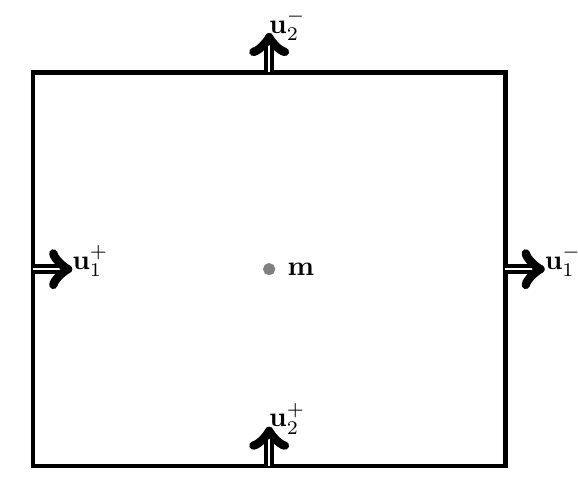
\begin{tikzpicture}[scale=1]
 	\draw[ultra thick]  (0,0) -- (6,0) -- (6,5) -- (0,5) -- cycle;
	\draw[black,ultra thick,double,->] (0,2.5) -- (0.5,2.5);
	\draw[black,ultra thick,double,->] (6,2.5) -- (6.5,2.5);
       \draw[black,ultra thick,double,->] (3,0) -- (3,0.5);
       \draw[black,ultra thick,double,->] (3,5) -- (3,5.5);
       
       %\draw[blue,ultra thick,double,->] (2,-2.5) -- (1,-2.7);
       %\draw[blue,ultra thick,double,->] (3.5,0) -- (3.5,1);
       %\draw[blue,ultra thick,double,->] (6,-2) -- (7,-2);
      \draw [gray,fill] (3,2.5) circle (2pt);
       \pgfputat{\pgfxy(3,2.5)}{\pgfbox[left,center]{\ \ $\bfm$}};
      \pgfputat{\pgfxy(0.5,2.6)}{\pgfbox[left,center]{$\bfu_{1}^{+}$}};
      \pgfputat{\pgfxy(6.5,2.6)}{\pgfbox[left,center]{$\bfu_{1}^{-}$}};
      
      \pgfputat{\pgfxy(3.0,0.6)}{\pgfbox[left,center]{$\bfu_{2}^{+}$}};
      \pgfputat{\pgfxy(3.0,5.6)}{\pgfbox[left,center]{$\bfu_{2}^{-}$}};
      

       \end{tikzpicture}
\caption{An example of a stagered grid cell with model parameters at the cell center and fluid velocity field on the edges. \label{fig:stag}}
\end{center}
\end{figure}

The  fluid velocity field $\bfu$ was  computed by solving equations \eqref{eq:flowp} and \eqref{eq:flowu} with a constant hydraulic conductivity for  $1$e$-03$ kg/s$^2$m$^2$. 
%
\begin{figure}[!h]
	\renewcommand{\arraystretch}{1.5}
	\begin{center}
		\iwidth=40mm	
		\begin{tabular}{|c|c|c|}
			\hline		
			 Tomography rays & Flow field\\	
			\hline				
			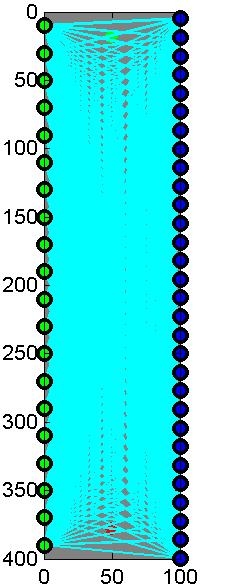
\includegraphics[width=1\iwidth]{figures/initialExperiment}
			&
			\includegraphics[width=1\iwidth]{figures/flow}\\			
			\hline
		\end{tabular}
	\end{center}
\caption{Initial experiment setup. Sources are pictured in green on the left and receivers in blue on. The initial setup covers the entire flow domain with 20 sources and 30 receivers.}
\label{fig:surveyDesign}
\end{figure}

\subsection{Regularization}
We chose a gradient operator for the linear regularization operator $\bfL = \GRADh$ to promote smoothness in the recovered models. The gradient maps from cell centers to edges with Dirichlet boundary conditions.

Two different inversions were carried out to recover models $\bfm_k$. First a linear inversion was performed with the gradient operator, and second a non-linear inversion was performed with smoothed total variation (TV) as the  regularization ~\cite{Ascher2006}. The total variation regularization promotes discontinuous boundaries, or sharp edges. This is particularly valid for our experiment since we have chosen advection without a diffusion term to transport a concentration of tracer. The tracer model is either 100\% concentrated in the blob and zero everywhere else. In this ideal case there should be no diffusion of the tracer, and thus the boundaries should remain sharp as it is advected along in the fluid velocity field.

In continuous space smoothed total variation is described by the following relation,
\begin{equation}
		R(m) = \alpha \int  \phi(|\grad |) \ d\vx.
\end{equation} 
A standard discrete 
approximation for the smoothed total variation regularization found in ~\cite{Ascher2006} is, 
\begin{equation}
\label{regsd}
R(\bfm) = \alpha h^2 \bfe^{\top} \sqrt{ \bfA_{f}^{c} \left( (\GRADh\ \bfm) \odot (\GRADh\ \bfm) \right)  + \epsilon},
\end{equation}
where the  gradient operator, $\GRADh$,   maps from cell centers to cell faces, and the averaging matrix $\bfA_{f}^{c}$ maps from faces to cell centers. 

Although we have formulated the optimal design based on a linear estimation of $\bfm$, it is not unreasonable to estimate $\bfm_k$ or $\bfm_0$ with a non-linear regularization, provided that this will contribute to recovering the best estimate of $\bfm_k$. As you can see in figure \ref{fig:erro1} below, the overall relative model error for the total variation regularization is significantly lower than that of the models recovered using the linear regularization. Thus the estimates obtained using the TV regularization are more accurate with respect to the true model for this problem. 
%
\begin{figure}[!h]
\begin{center}
\iwidth=180mm
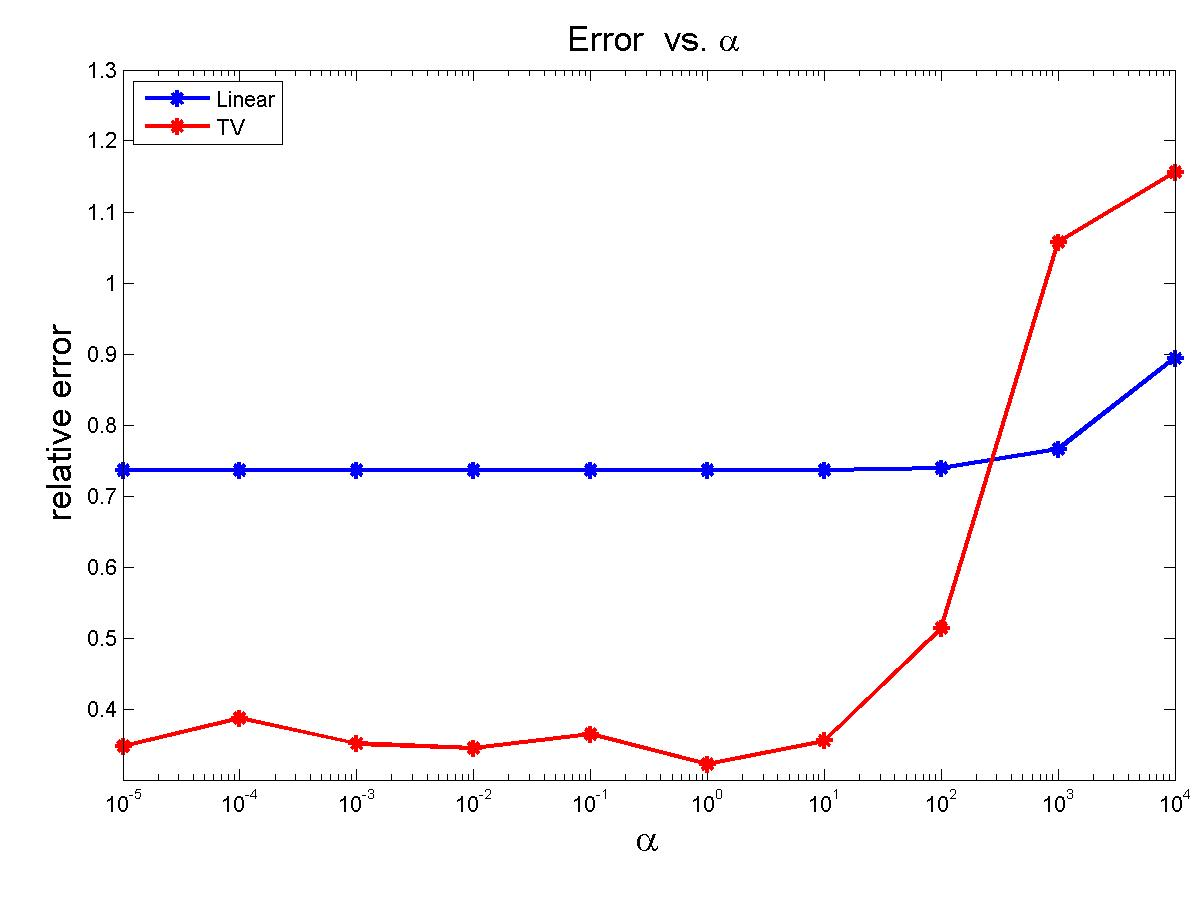
\includegraphics[width=.75\iwidth]{figures/newFigs/exp2-error1}
\end{center}
\caption{Plot of the relative error ($\|\bfm_1^{true}-\bfmhat_1\|/(    \|\bfm^{true}_1\|)$) versus the regularization parameter $\alpha$ for both the linear regularization and smoothed total variation. }
	\label{fig:erro1}
\end{figure} 

\todo[inline]{ I'm not super happy with this figure...it's just to illustrate the hand wavy argument about using different regularizations to reconstruct m's. }








\subsection{Monitor function}
We chose the binary monitor function 
\begin{equation*}
\bftau_{B} =  
\begin{cases}
0, & \text{if } \bfdelta \leq 0\\
1, & \text{if } \bfdelta > 0
\end{cases}
\end{equation*}
where $\bfdelta = \bfm_{k} -\bfm_{\text{background}} $ to provide historic data to the adaptive A-optimal design problem. The background model $\bfm_{\text{background}} $, is the same model used to compute the velocity field in equation \eqref{eq:flowu}. In other words, we are designing only to track the target instead of fully imaging the entire domain. 

\section{Design results: Noiseless dynamics}
\label{sec:Results}
To generate data, the initial tracer concentration was marched along in time for time steps of 25 days and measured by conducting a tomography survey at each time with Gaussian noise added to each data set. In total 9 experiments were conducted for times $t_0,t_1,...,t_8$. 



The initial design for time point $t_0$ did not include the dynamics. This amounts to  setting $\bftau_0 = 1$ in algorithm \ref{algo1}. The design algorithm is therefore identical to the static case and produces an optimal design based on the physics and that of the linear regularization operator $\bfL$, without any historic data. This is apparent in both the plot of the weights for experiment 1 at time  $t_0$ in figure \ref{fig:weights1} and the image of the rays in figure \ref{fig:results1}, where the design specifies fewer rays that cover the entire domain. In other words, the design algorithm has no information about the location of the target at this point. 

For each experiment the {\sf amse} was plotted versus the number of nonzero weights for a set of regularization parameters $\beta$, see figure \ref{fig:weights1} for examples for times $t_0,t_2,t_4$. From these curves, the best set of weights were chosen such that the weights were sparse, but also so the {\sf amse} was kept reasonably small. The experiment weights are also plotted. 
\begin{figure}[!h]
	\renewcommand{\arraystretch}{1.5}
	\begin{center}
		\iwidth=80mm
		\begin{tabular}{|c|c|c|} %{@{}|@{\ }p{3mm}@{}|@{\ }c@{\;}|@{\;}c@{\ }|}
			\hline		
			Exp & Sparsity & Weights	\\
			\hline	
			$t_0$
			&	
			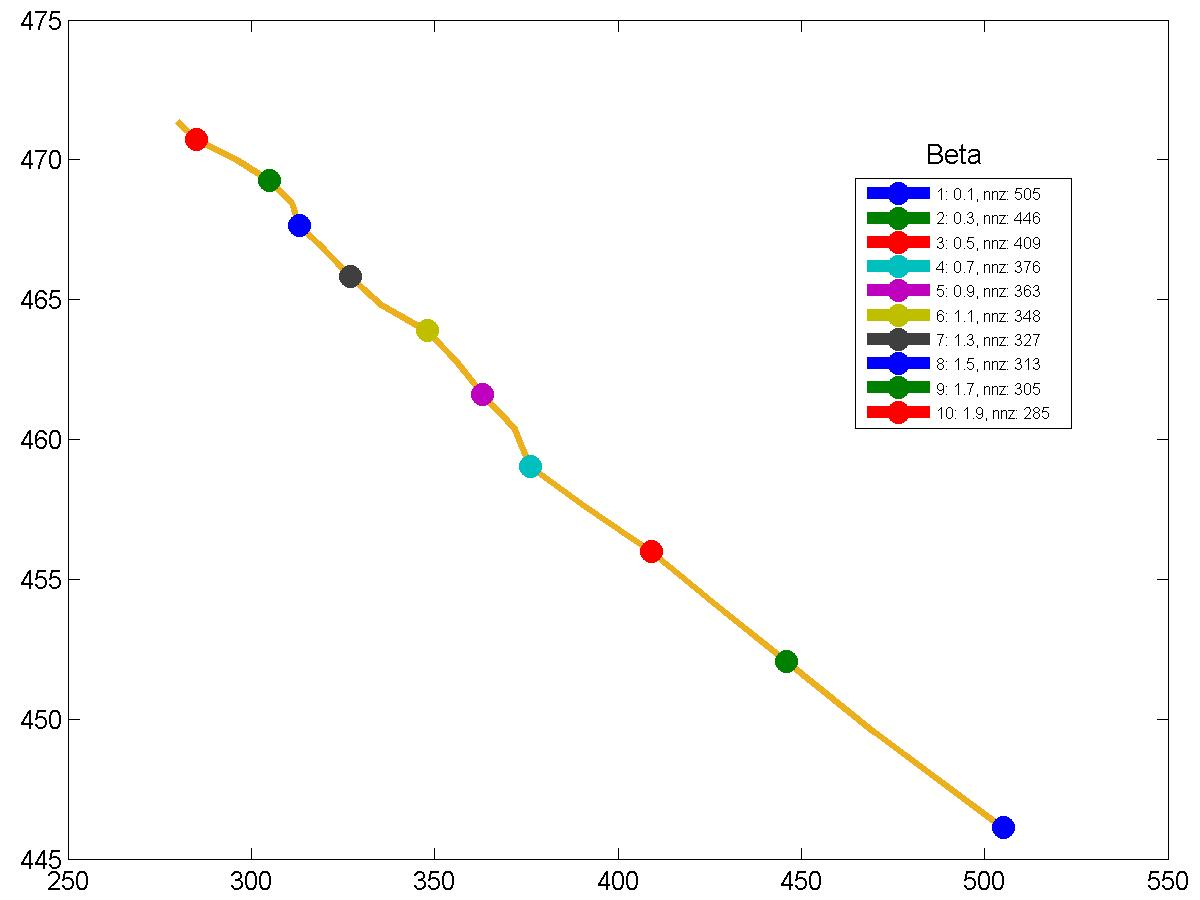
\includegraphics[width=.8\iwidth]{figures/newFigs/exp1paretoWeights}
			&
			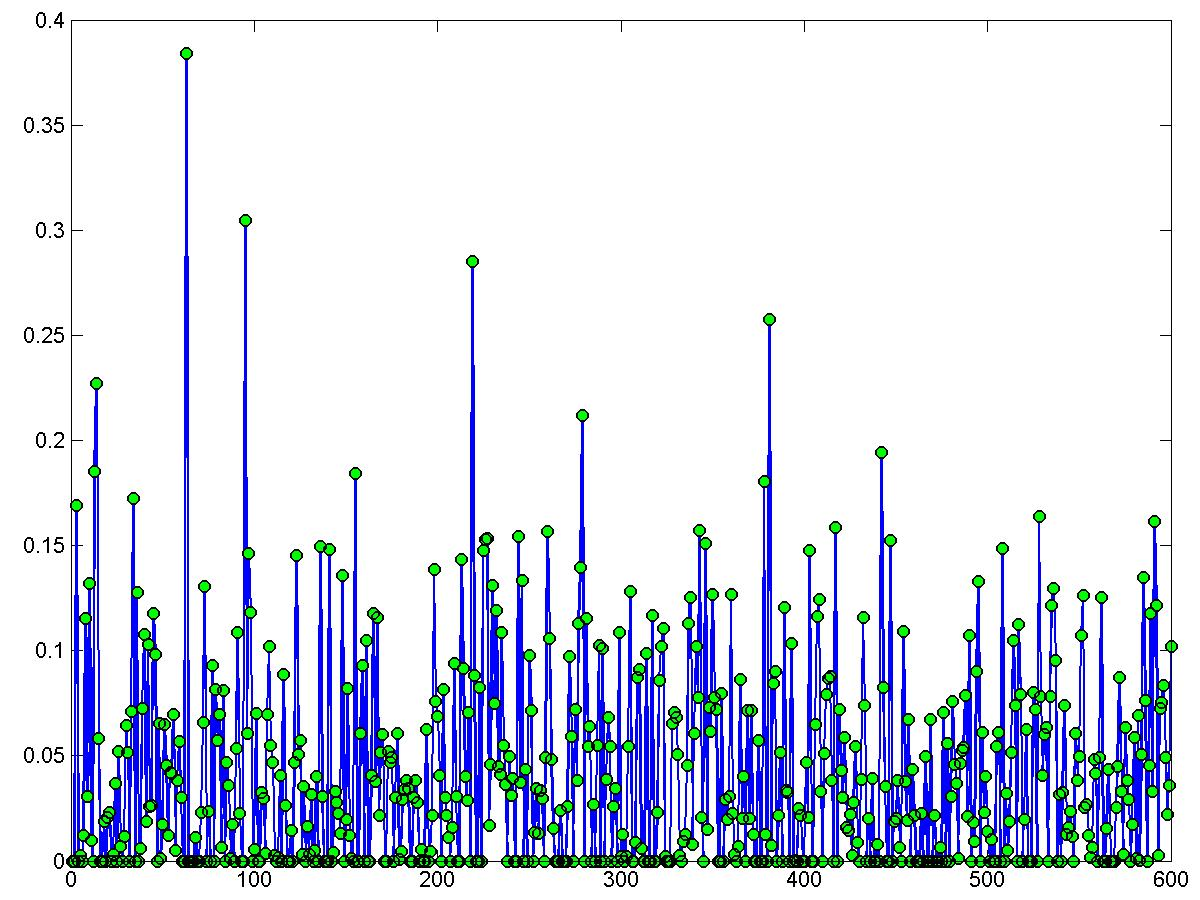
\includegraphics[width=.8\iwidth]{figures/newFigs/exp1Weights}\\
			\hline
			$t_2$
			&	
			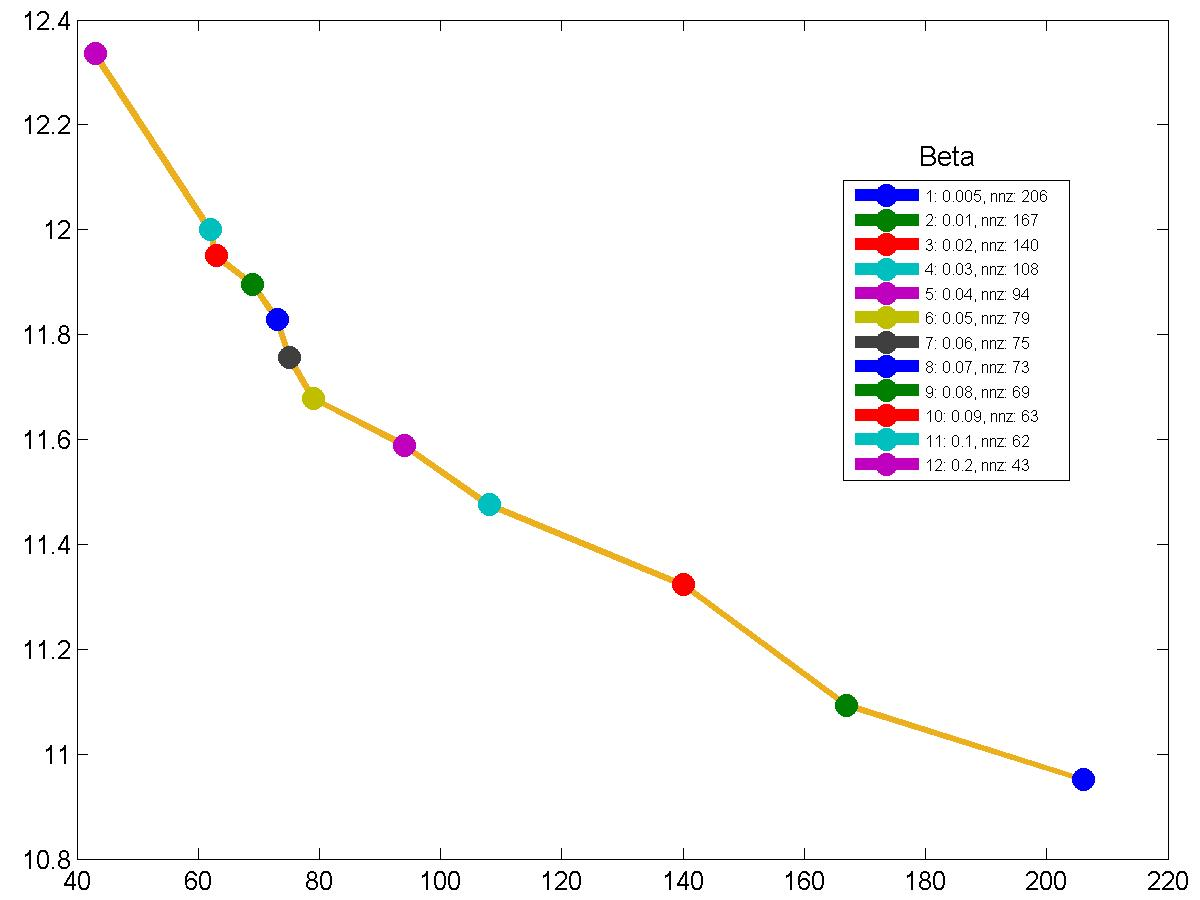
\includegraphics[width=.8\iwidth]{figures/newFigs/exp3paretoWeights}
			&
			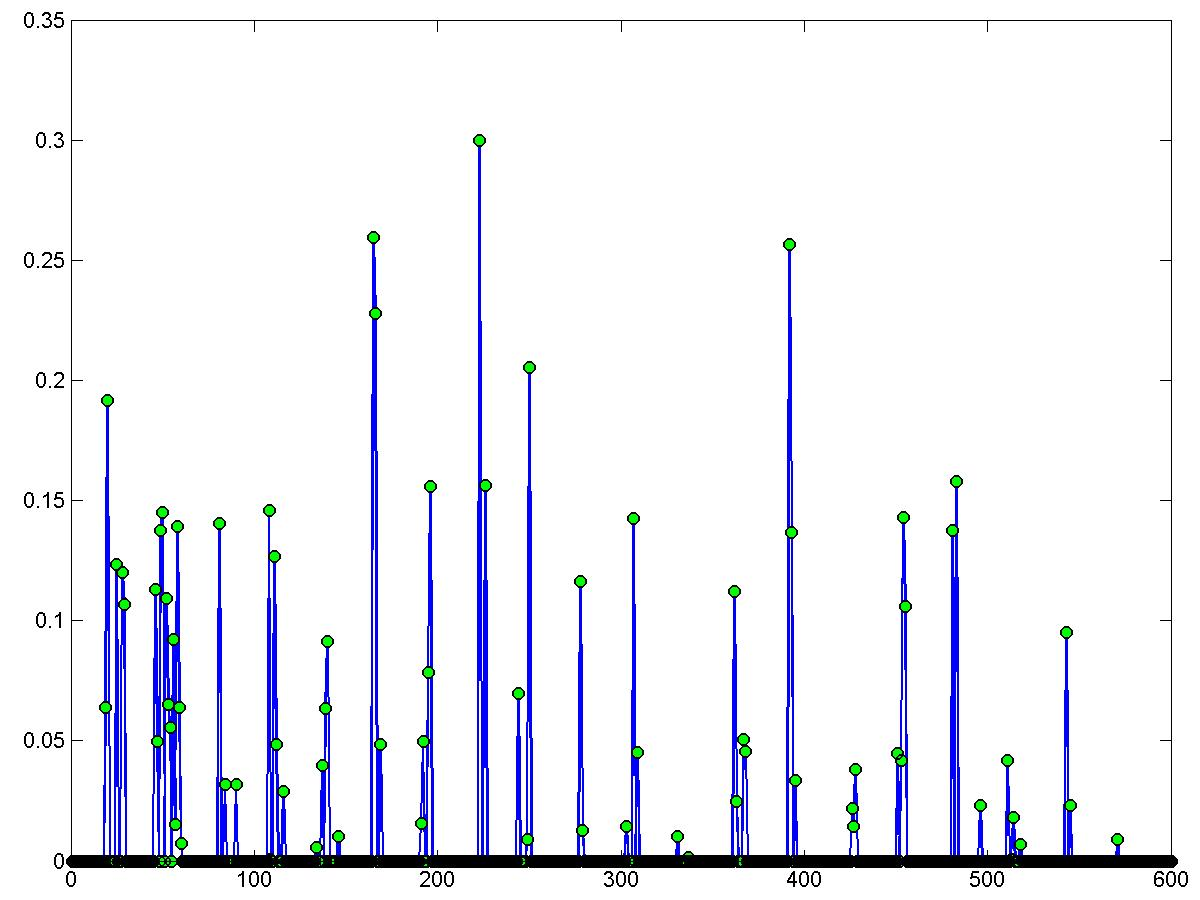
\includegraphics[width=.8\iwidth]{figures/newFigs/exp3Weights}\\
			\hline
			$t_4$
			&	
			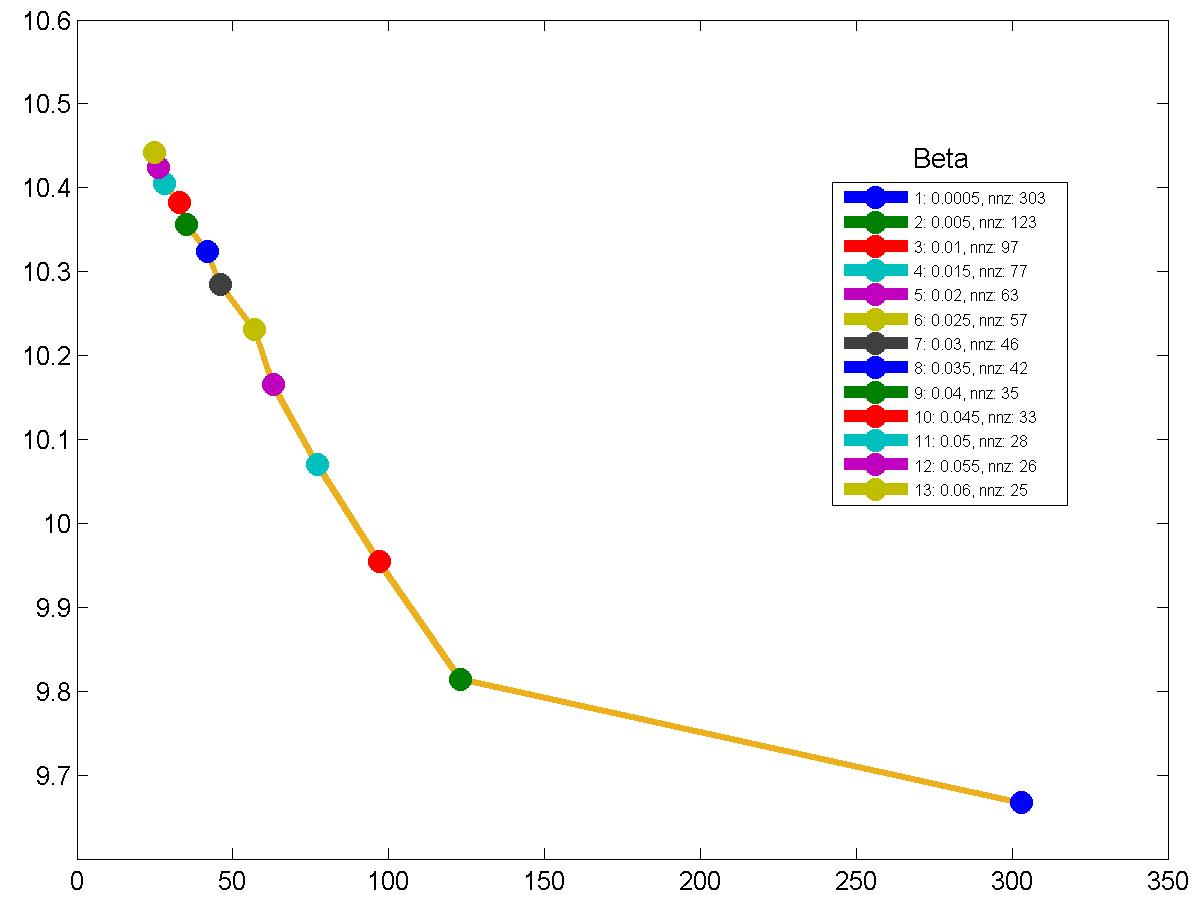
\includegraphics[width=.8\iwidth]{figures/newFigs/exp5paretoWeights}
			&
			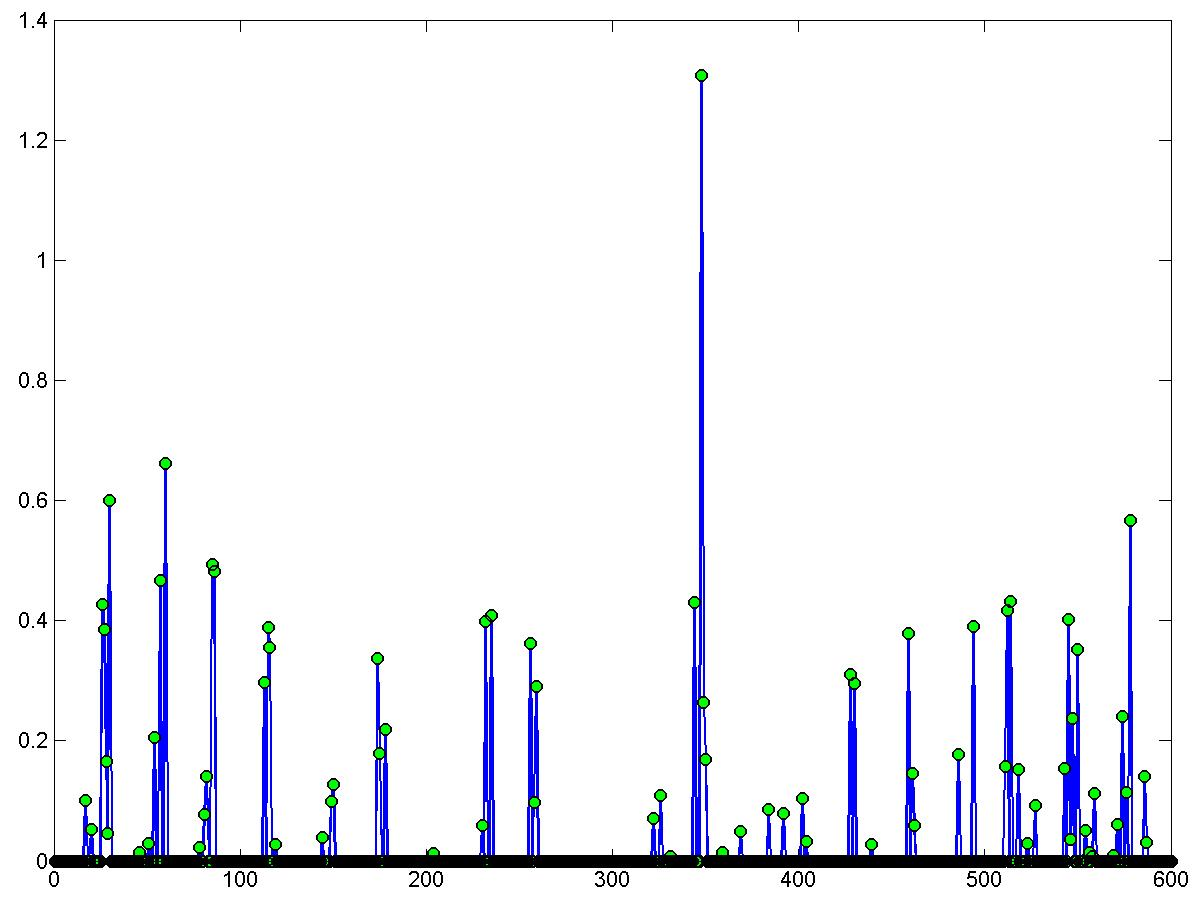
\includegraphics[width=.8\iwidth]{figures/newFigs/exp5Weights}\\			
			\hline
		\end{tabular}
	\end{center}
	\caption{Noiseless dynamics: Plots of the {\sf amse} vs. the number of nonzero weights (left column), and the weights used to conduct the experiment for experiments 1,3,and 5, at times $t_0,t_2,t_4$.}
	\label{fig:weights1}
\end{figure}

After each each experimental design was determined, both $\bfm_0$ and the current model $\bfm_k$ were reconstructed from the reduced set of data corresponding to the optimal experimental design. The new estimate for $\bfm_0$ was then used to compute $\bftau_k$. In figure \ref{fig:results1} the rays corresponding to the optimal experimental design data used to estimate the current models are pictured in blue over an image of the model. Note that the rays tend to follow the target as it moves through the domain, and rays which do not pass through the target are not included in the design.  The total number of data required to image the models is significantly reduced. In most cases the number of data are approximately 40 of a possible 600. There do appear to be some rays that do not pass through the target that are included in the optimal design, and thus would not contribute to the image reconstruction. However, since the reconstruction of $\bfm_0$ is never perfect and there is noise in the data, these spurious rays are expected. 

It is also apparent that the number of spurious rays increases further in time. In particular, at time $t_6$ it appears that the design algorithm has a harder time generating a design that captures the target well. There are many more rays which do not pass through the target. This is likely due to the increasing number of multiplications by the transport matrix $\bfT$ as time progresses. This is by no means a perfect process.

It is also apparent in the reconstructions of $\bfm_k$ with smoothed total variation regularization does a better job, even when the optimal design was computed for the linear regularization model estimation problem. Again, this is to be expected since we have chosen a model with discontinuous edges, and are transporting the target only by advection. 
\begin{figure}[!h]
	\renewcommand{\arraystretch}{1.5}
	\begin{center}
		\iwidth=13mm
		\begin{tabular}{|c|c|c|c|c|c|c|c|c|}
			\hline		
			 exp $t_0$ & exp $t_1$ & exp $t_2$& exp $t_3$& exp $t_4$& exp $t_5$& exp $t_6$ & exp $t_7$ & exp $t_8$\\
			\hline		
			\includegraphics[width=.9\iwidth]{figures/newFigs/resultsExp-1-designs}
			&
			\includegraphics[width=.9\iwidth]{figures/newFigs/resultsExp-2-designs}
			&
			\includegraphics[width=.9\iwidth]{figures/newFigs/resultsExp-3-designs}
			&
			\includegraphics[width=.9\iwidth]{figures/newFigs/resultsExp-4-designs}
			&
			\includegraphics[width=.9\iwidth]{figures/newFigs/resultsExp-5-designs}
			&
			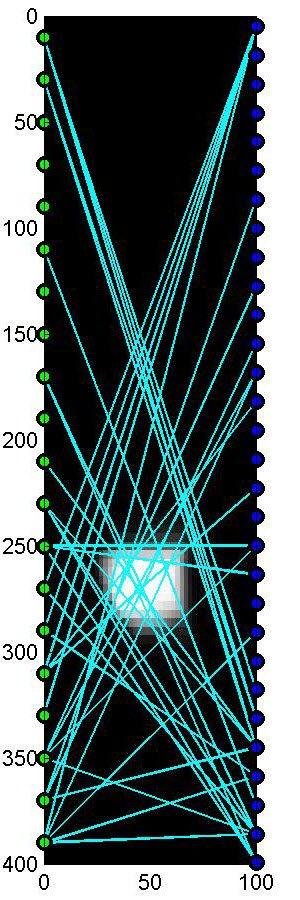
\includegraphics[width=.9\iwidth]{figures/newFigs/resultsExp-6-designs}
			&
			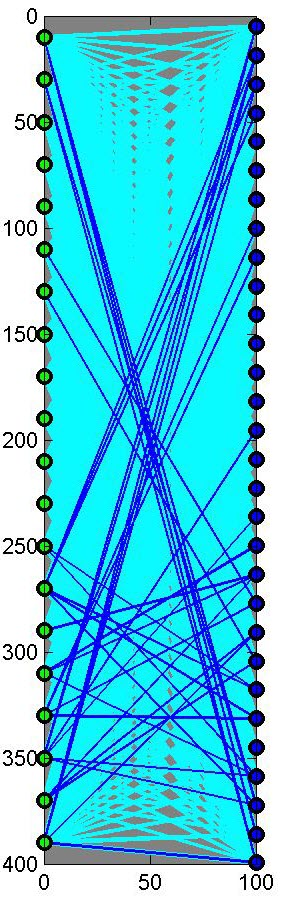
\includegraphics[width=.9\iwidth]{figures/newFigs/resultsExp-7-designs}
			&
			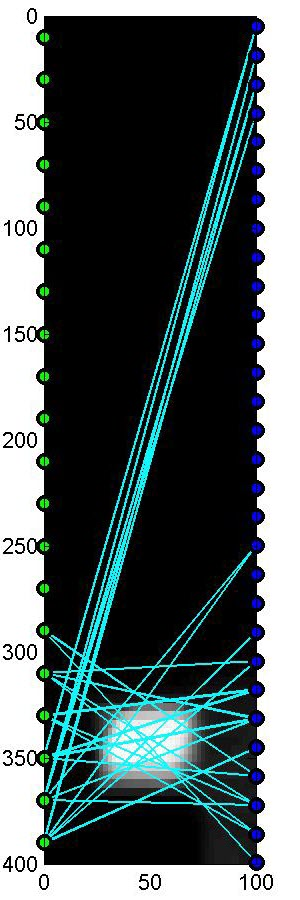
\includegraphics[width=.9\iwidth]{figures/newFigs/resultsExp-8-designs}
			&
			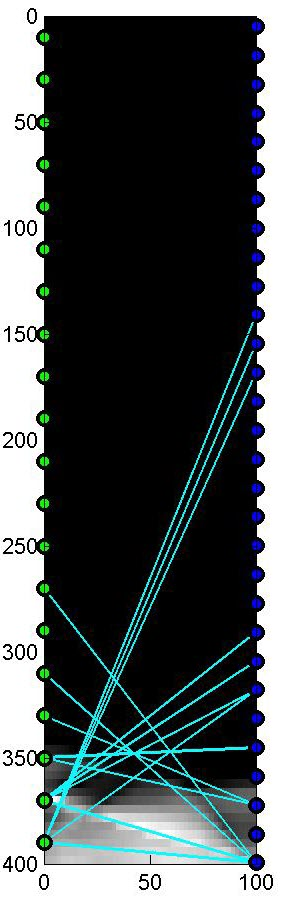
\includegraphics[width=.9\iwidth]{figures/newFigs/resultsExp-9-designs}			
			\\
			\hline
			$\#d=350$& $\#d=43$& $\#d=46$& $\#d= 57$& $\#d=35$& $\#d=35$& $\#d=30$& $\#d=25$& $\# d=19$\\
			\hline	
			 $\bfm^{\sf True}_{t_0}$& $\bfm^{\sf True}_{t_1}$&$\bfm^{\sf True}_{t_2}$& $\bfm^{\sf True}_{t_3}$&$\bfm^{\sf True}_{t_4}$& $\bfm^{\sf True}_{t_5}$ &$\bfm^{\sf True}_{t_6}$&$\bfm^{\sf True}_{t_7}$& $\bfm^{\sf True}_{t_8}$ 
			 \\
			\hline	
			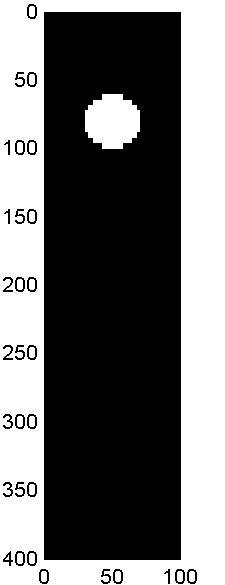
\includegraphics[width=.9\iwidth]{figures/newFigs/resultsExp-1-mtrue}
			&
			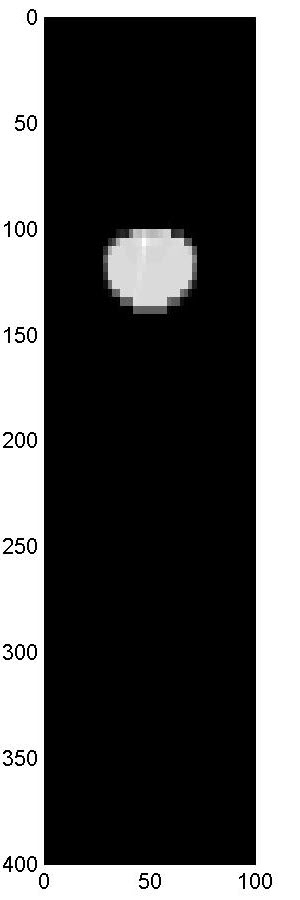
\includegraphics[width=.9\iwidth]{figures/newFigs/resultsExp-2-mtrue}
			&
			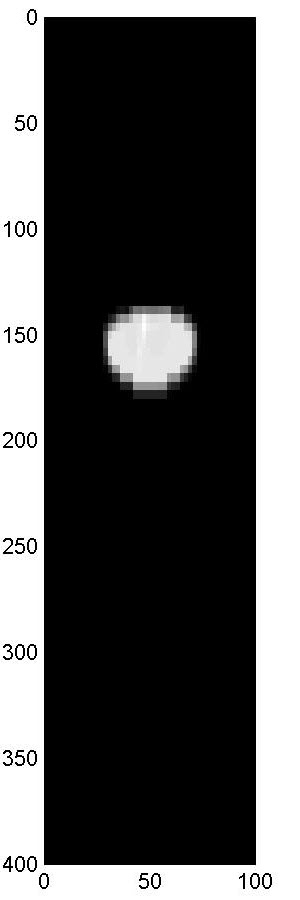
\includegraphics[width=.9\iwidth]{figures/newFigs/resultsExp-3-mtrue}
			&
			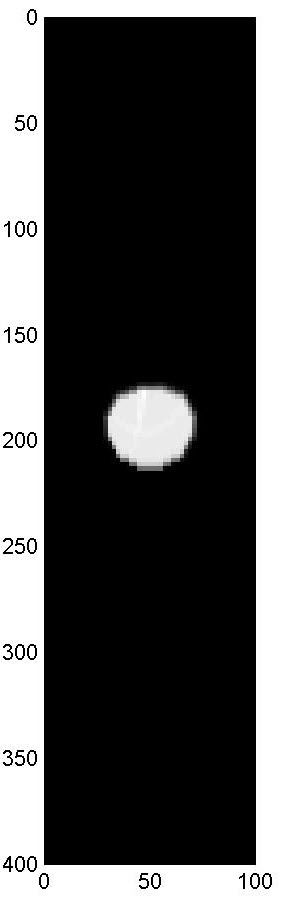
\includegraphics[width=.9\iwidth]{figures/newFigs/resultsExp-4-mtrue}
			&
			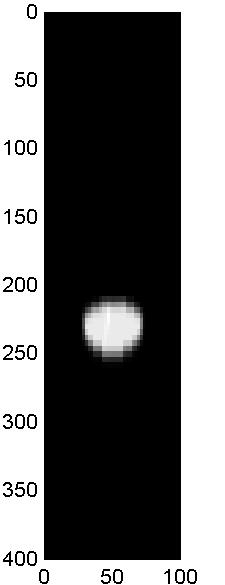
\includegraphics[width=.9\iwidth]{figures/newFigs/resultsExp-5-mtrue}
			&
			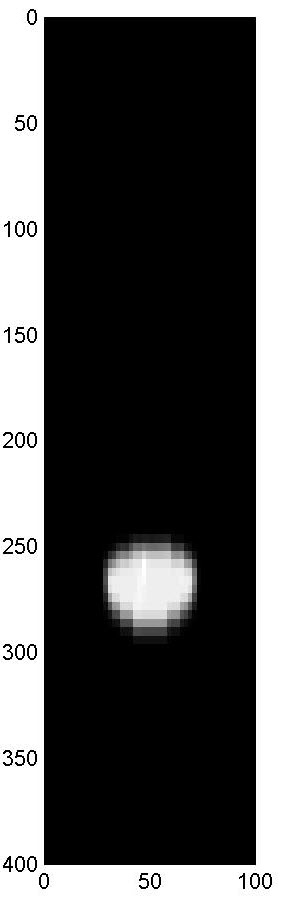
\includegraphics[width=.9\iwidth]{figures/newFigs/resultsExp-6-mtrue}
			&
			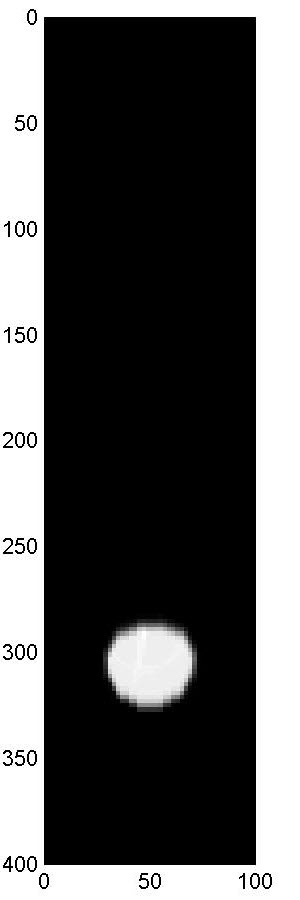
\includegraphics[width=.9\iwidth]{figures/newFigs/resultsExp-7-mtrue}
			&
			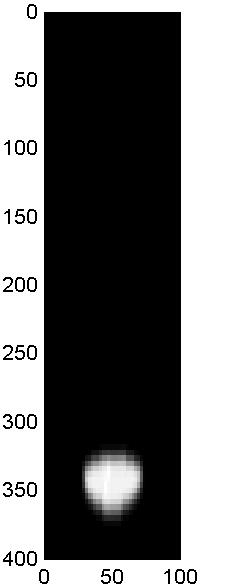
\includegraphics[width=.9\iwidth]{figures/newFigs/resultsExp-8-mtrue}
			&
			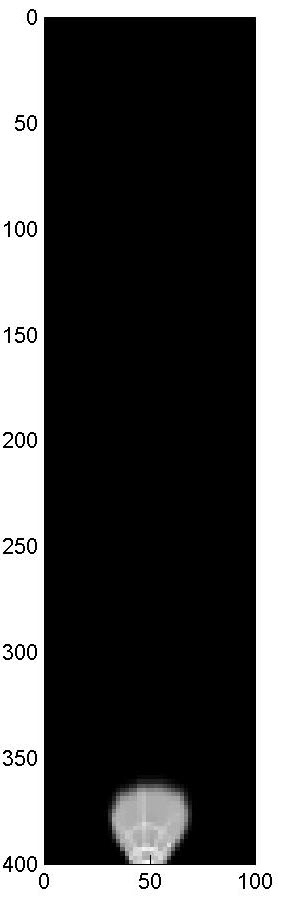
\includegraphics[width=.9\iwidth]{figures/newFigs/resultsExp-9-mtrue}
			\\
			\hline
			 $\bfm^{\sf TV}_{t_0}$& $\bfm^{\sf TV}_{t_1}$&$\bfm^{\sf TV}_{t_2}$& $\bfm^{\sf TV}_{t_3}$&$\bfm^{\sf TV}_{t_4}$& $\bfm^{\sf TV}_{t_5}$ &$\bfm^{\sf TV}_{t_6}$&$\bfm^{\sf TV}_{t_7}$& $\bfm^{\sf TV}_{t_8}$ \\
			\hline	
			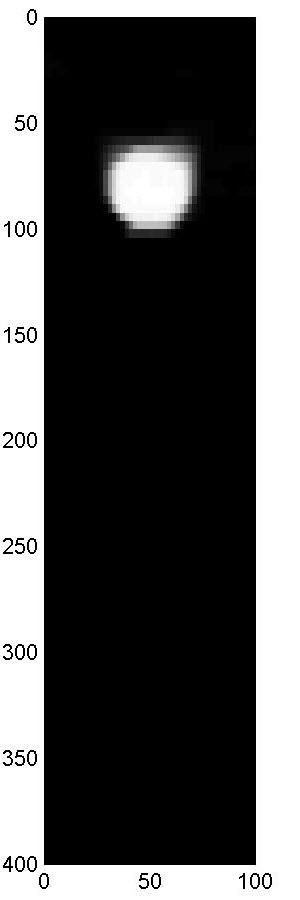
\includegraphics[width=.9\iwidth]{figures/newFigs/resultsExp-1-mkTV}
			&
			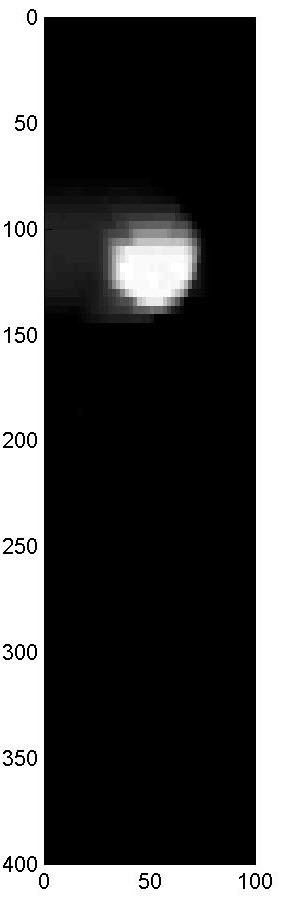
\includegraphics[width=.9\iwidth]{figures/newFigs/resultsExp-2-mkTV}
			&
			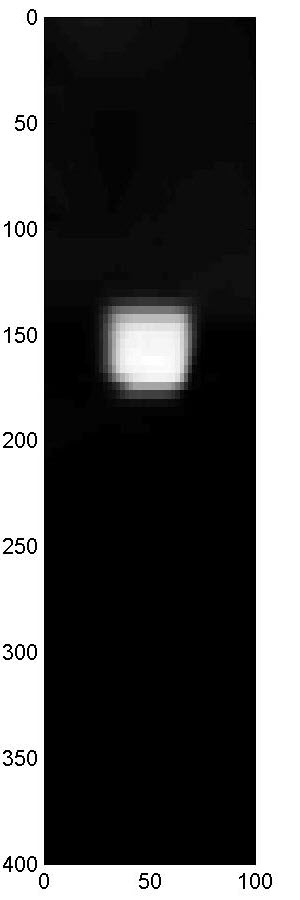
\includegraphics[width=.9\iwidth]{figures/newFigs/resultsExp-3-mkTV}
			&
			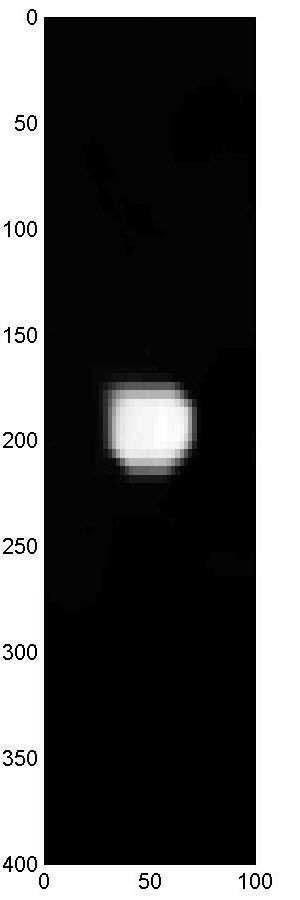
\includegraphics[width=.9\iwidth]{figures/newFigs/resultsExp-4-mkTV}
			&
			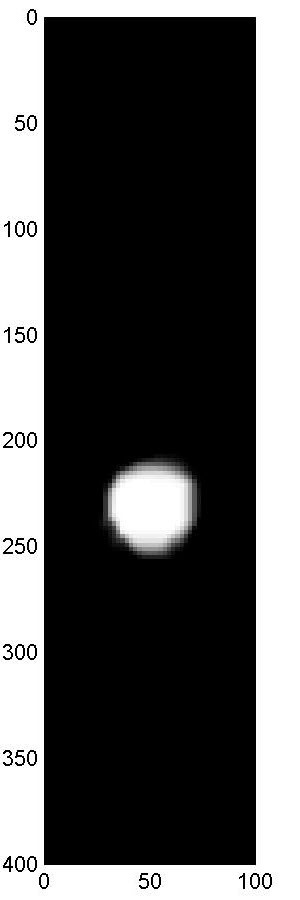
\includegraphics[width=.9\iwidth]{figures/newFigs/resultsExp-5-mkTV}
			&
			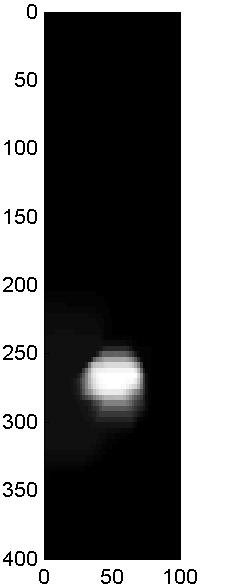
\includegraphics[width=.9\iwidth]{figures/newFigs/resultsExp-6-mkTV}
			&
			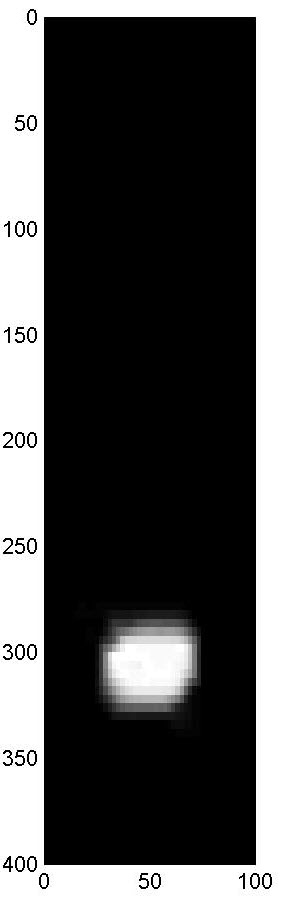
\includegraphics[width=.9\iwidth]{figures/newFigs/resultsExp-7-mkTV}
			&
			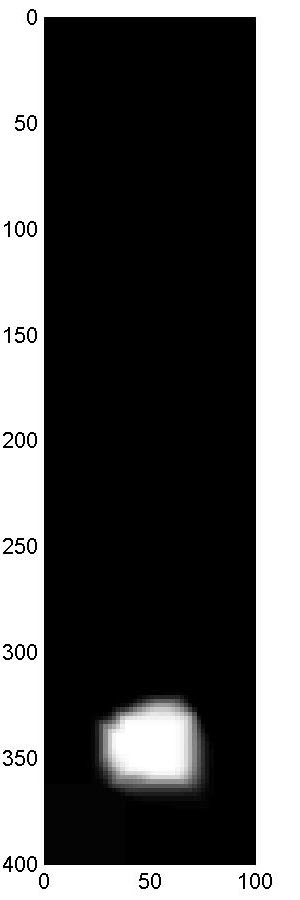
\includegraphics[width=.9\iwidth]{figures/newFigs/resultsExp-8-mkTV}
			&
			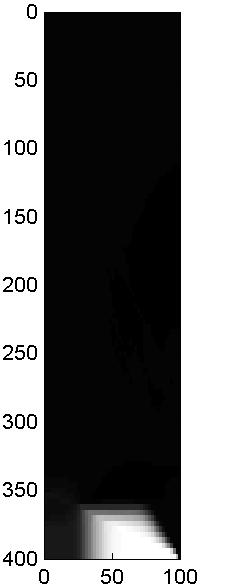
\includegraphics[width=.9\iwidth]{figures/newFigs/resultsExp-9-mkTV}
			\\
			\hline	
			 $\bfm^{\sf Lin}_{t_0}$& $\bfm^{\sf Lin}_{t_1}$&$\bfm^{\sf Lin}_{t_2}$& $\bfm^{\sf Lin}_{t_3}$&$\bfm^{\sf Lin}_{t_4}$& $\bfm^{\sf Lin}_{t_5}$ &$\bfm^{\sf Lin}_{t_6}$&$\bfm^{\sf Lin}_{t_7}$& $\bfm^{\sf Lin}_{t_8}$ \\
			\hline	
			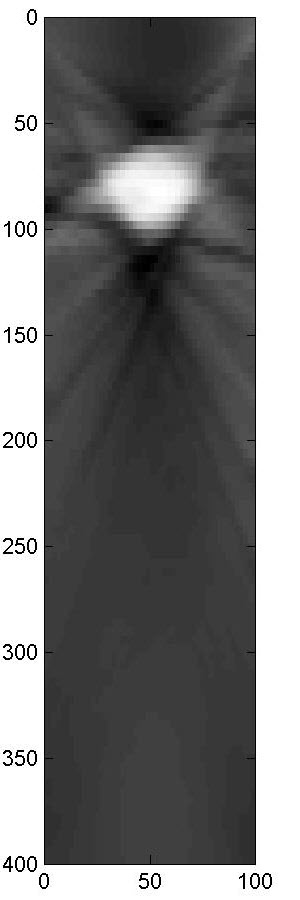
\includegraphics[width=.9\iwidth]{figures/newFigs/resultsExp-1-mk}
			&
			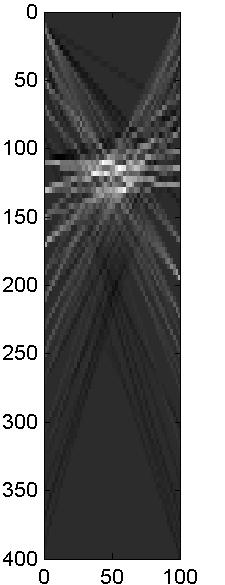
\includegraphics[width=.9\iwidth]{figures/newFigs/resultsExp-2-mk}
			&
			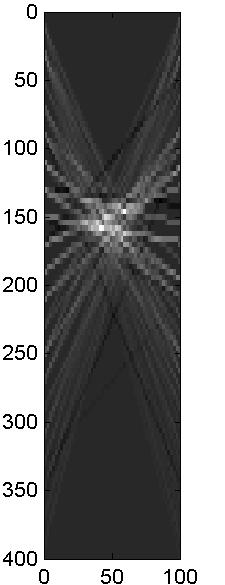
\includegraphics[width=.9\iwidth]{figures/newFigs/resultsExp-3-mk}
			&
			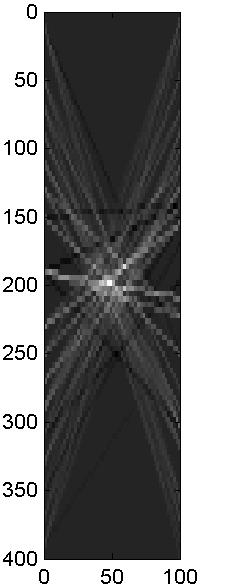
\includegraphics[width=.9\iwidth]{figures/newFigs/resultsExp-4-mk}
			&
			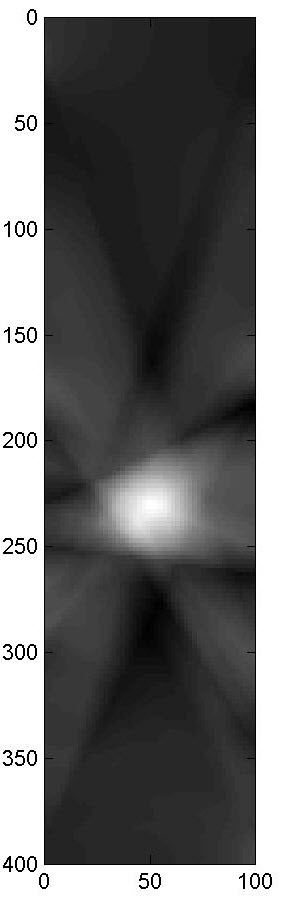
\includegraphics[width=.9\iwidth]{figures/newFigs/resultsExp-5-mk}
			&
			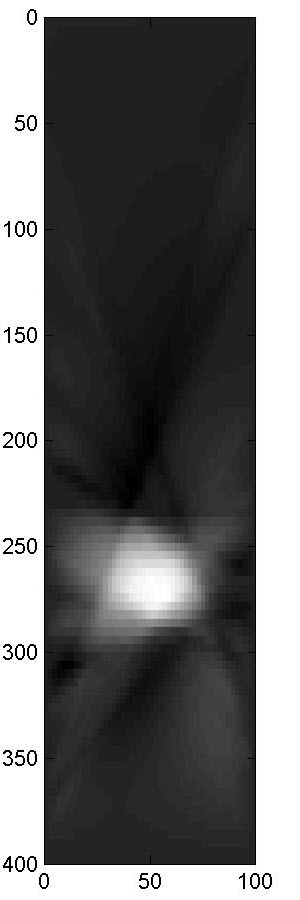
\includegraphics[width=.9\iwidth]{figures/newFigs/resultsExp-6-mk}
			&
			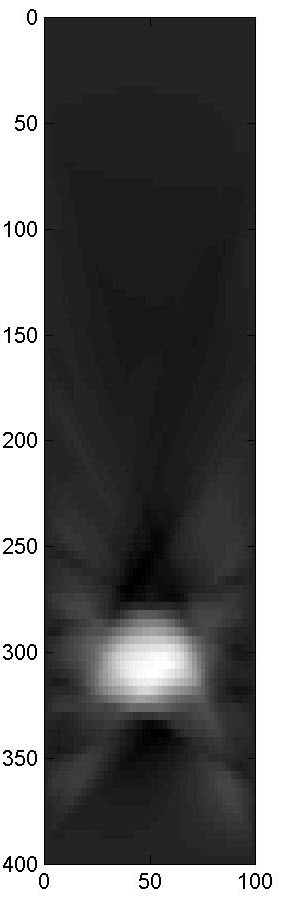
\includegraphics[width=.9\iwidth]{figures/newFigs/resultsExp-7-mk}
			&
			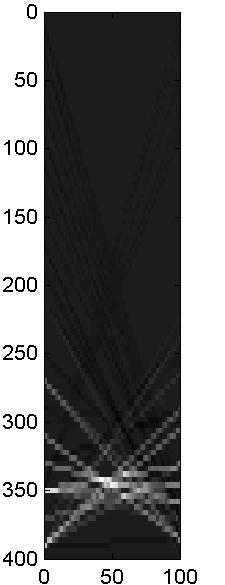
\includegraphics[width=.9\iwidth]{figures/newFigs/resultsExp-8-mk}
			&
			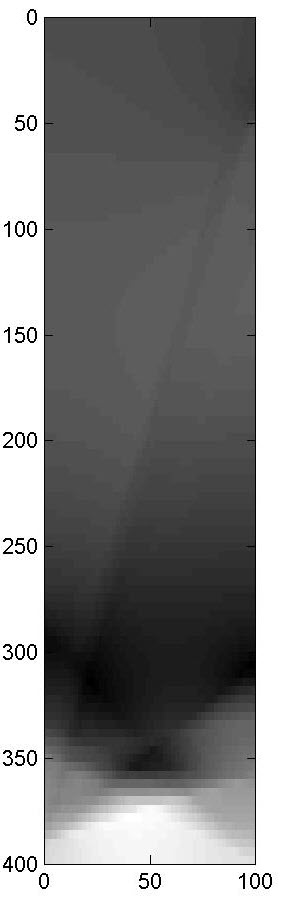
\includegraphics[width=.9\iwidth]{figures/newFigs/resultsExp-9-mk}		
			\\			
			\hline
		\end{tabular}
	\end{center}
	\caption{Noiseless dynamics: Optimal designs and recovered models for 9 experiments. The top row shows the rays and the recovered model, with the number of rays (\#d = 350) given below, followed by the true models, the models recovered using total variation, and finally the models recovered using the linear gradient regularization.}
	\label{fig:results1}
\end{figure}


\section{Results: Noisy  dynamics}
\label{sec: Example2}
To demonstrate the adaptive method for the noisy formulation presented in section \ref{sec:Noisy},  the tracer target was  marched along in time while determining an optimal survey design for the future experiment given all historic data. For the first experiment $\bfw_0$, the initial naive experiment computed in the noiseless example was used. Each model was reconstructed at each time step using the reduced data sets determined by the optimal design. Models were reconstructed using the non-linear smoothed total variation regularization, and also with the linear regularization. 
The covariance matrices $\bfQ_k$ were set as a scale $\alpha_k \bfI$ for the initial experiment, where $\alpha_k= 10^{-8}$. 

The results are pictured in figure \ref{fig:results2}, below. It is apparent that we were again able to track the motion of the target with a significantly reduced set of measurements. However, in this case the overall number of rays passing through the target were higher than that of the noiseless formulation. There also appear to be less  spurious rays. The recoveries for $\bfm_k$ using the linear regularization term approximate the true models to a better extent that those of the noiseless formulation. 

Unfortunately although the designs appear to be more accurate in this case, the computation time is significantly longer than the noiseless formulation. This is particularly true if the full system is formed instead of using GMRES to solve the big systems for all of the $\bfz$'s. 


\todo[inline]{Things to quantify - relative data fit error. Also should comment on computation time? The noiseless method is faster. For the noisy case I solved it two ways, building the whole system and using backslash, or not forming anything and using gmres. Both are slow. Debating on leaving this as a qualitative explanation vs. actually quoting some numbers...Thoughts Eldad?}

\begin{figure}[!h]
	\renewcommand{\arraystretch}{1.5}
	\begin{center}
		\iwidth=13mm
		\begin{tabular}{|c|c|c|c|c|c|c|c|c|}
			\hline		
			 exp $t_0$ & exp $t_1$ & exp $t_2$& exp $t_3$& exp $t_4$& exp $t_5$& exp $t_6$ & exp $t_7$ & exp $t_8$\\
			\hline		
			\includegraphics[width=.9\iwidth]{figures/newFigs/noisy/resultsExp-1-designs}
			&
			\includegraphics[width=.9\iwidth]{figures/newFigs/noisy/resultsExp-2-designs}
			&
			\includegraphics[width=.9\iwidth]{figures/newFigs/noisy/resultsExp-3-designs}
			&
			\includegraphics[width=.9\iwidth]{figures/newFigs/noisy/resultsExp-4-designs}
			&
			\includegraphics[width=.9\iwidth]{figures/newFigs/noisy/resultsExp-5-designs}
			&
			\includegraphics[width=.9\iwidth]{figures/newFigs/noisy/resultsExp-6-designs}
			&
			\includegraphics[width=.9\iwidth]{figures/newFigs/noisy/resultsExp-7-designs}
			&
			\includegraphics[width=.9\iwidth]{figures/newFigs/noisy/resultsExp-8-designs}
			&
			\includegraphics[width=.9\iwidth]{figures/newFigs/noisy/resultsExp-9-designs}			
			\\
			\hline
			$\#d=297$& $\#d=58$& $\#d=62$& $\#d= 77$& $\#d=65$& $\#d=65$& $\#d=81$& $\#d=54$& $\# d=14$\\
			\hline	
			 $\bfm^{\sf True}_{t_0}$& $\bfm^{\sf True}_{t_1}$&$\bfm^{\sf True}_{t_2}$& $\bfm^{\sf True}_{t_3}$&$\bfm^{\sf True}_{t_4}$& $\bfm^{\sf True}_{t_5}$ &$\bfm^{\sf True}_{t_6}$&$\bfm^{\sf True}_{t_7}$& $\bfm^{\sf True}_{t_8}$ 
			 \\
			\hline	
			\includegraphics[width=.9\iwidth]{figures/newFigs/noisy/resultsExp-1-mtrue}
			&
			\includegraphics[width=.9\iwidth]{figures/newFigs/noisy/resultsExp-2-mtrue}
			&
			\includegraphics[width=.9\iwidth]{figures/newFigs/noisy/resultsExp-3-mtrue}
			&
			\includegraphics[width=.9\iwidth]{figures/newFigs/noisy/resultsExp-4-mtrue}
			&
			\includegraphics[width=.9\iwidth]{figures/newFigs/noisy/resultsExp-5-mtrue}
			&
			\includegraphics[width=.9\iwidth]{figures/newFigs/noisy/resultsExp-6-mtrue}
			&
			\includegraphics[width=.9\iwidth]{figures/newFigs/noisy/resultsExp-7-mtrue}
			&
			\includegraphics[width=.9\iwidth]{figures/newFigs/noisy/resultsExp-8-mtrue}
			&
			\includegraphics[width=.9\iwidth]{figures/newFigs/noisy/resultsExp-9-mtrue}
			\\
			\hline
			 $\bfm^{\sf TV}_{t_0}$& $\bfm^{\sf TV}_{t_1}$&$\bfm^{\sf TV}_{t_2}$& $\bfm^{\sf TV}_{t_3}$&$\bfm^{\sf TV}_{t_4}$& $\bfm^{\sf TV}_{t_5}$ &$\bfm^{\sf TV}_{t_6}$&$\bfm^{\sf TV}_{t_7}$& $\bfm^{\sf TV}_{t_8}$ \\
			\hline	
			\includegraphics[width=.9\iwidth]{figures/newFigs/noisy/resultsExp-1-mkTV}
			&
			\includegraphics[width=.9\iwidth]{figures/newFigs/noisy/resultsExp-2-mkTV}
			&
			\includegraphics[width=.9\iwidth]{figures/newFigs/noisy/resultsExp-3-mkTV}
			&
			\includegraphics[width=.9\iwidth]{figures/newFigs/noisy/resultsExp-4-mkTV}
			&
			\includegraphics[width=.9\iwidth]{figures/newFigs/noisy/resultsExp-5-mkTV}
			&
			\includegraphics[width=.9\iwidth]{figures/newFigs/noisy/resultsExp-6-mkTV}
			&
			\includegraphics[width=.9\iwidth]{figures/newFigs/noisy/resultsExp-7-mkTV}
			&
			\includegraphics[width=.9\iwidth]{figures/newFigs/noisy/resultsExp-8-mkTV}
			&
			\includegraphics[width=.9\iwidth]{figures/newFigs/noisy/resultsExp-9-mkTV}
			\\
			\hline	
			 $\bfm^{\sf Lin}_{t_0}$& $\bfm^{\sf Lin}_{t_1}$&$\bfm^{\sf Lin}_{t_2}$& $\bfm^{\sf Lin}_{t_3}$&$\bfm^{\sf Lin}_{t_4}$& $\bfm^{\sf Lin}_{t_5}$ &$\bfm^{\sf Lin}_{t_6}$&$\bfm^{\sf Lin}_{t_7}$& $\bfm^{\sf Lin}_{t_8}$ \\
			\hline	
			\includegraphics[width=.9\iwidth]{figures/newFigs/noisy/resultsExp-1-mk}
			&
			\includegraphics[width=.9\iwidth]{figures/newFigs/noisy/resultsExp-2-mk}
			&
			\includegraphics[width=.9\iwidth]{figures/newFigs/noisy/resultsExp-3-mk}
			&
			\includegraphics[width=.9\iwidth]{figures/newFigs/noisy/resultsExp-4-mk}
			&
			\includegraphics[width=.9\iwidth]{figures/newFigs/noisy/resultsExp-5-mk}
			&
			\includegraphics[width=.9\iwidth]{figures/newFigs/noisy/resultsExp-6-mk}
			&
			\includegraphics[width=.9\iwidth]{figures/newFigs/noisy/resultsExp-7-mk}
			&
			\includegraphics[width=.9\iwidth]{figures/newFigs/noisy/resultsExp-8-mk}
			&
			\includegraphics[width=.9\iwidth]{figures/newFigs/noisy/resultsExp-9-mk}		
			\\			
			\hline
		\end{tabular}
	\end{center}
	\caption{Noisey dynamics: Optimal designs and recovered models for 9 experiments. The top row shows the rays and the recovered model, with the number of rays (ex. \#d = 297) given below. The second row pictures true models, the third shows the  models recovered using total variation, and finally the bottom shows models recovered using the linear gradient regularization.}
	\label{fig:results2}
\end{figure}


\section{Concluding remarks}
In this paper we have presented a new method for the design of experiments for a dynamic target which incorporates historic data. Our approach is based on coupling the dynamic governing partial differential equation with the geophysical imaging partial differential equation to estimate model parameters, and the introduction of a monitor function to scale the posterior mean squared error (amse) according to historic model estimators. Our optimal design approach  minimizes the amse to determine an optimal experimental design for a future experiment. 
As a result of this method, optimal designs are conditioned on the both the physics of the problem and historic data. This leads to designs which track the motion of the target, and estimation of the tagret that require a minimum number of data points. 
\bibliographystyle{plain}
\bibliography{designBib}
%\bibliography{../../../../Biblio/biblio}
\end{document}


